\chapter{Dynamic Maps}
\label{chap:dcm}

\bibentry{mcnabb2018dynamic} \cite{mcnabb2018dynamic} \\

\chapterquote{A problem of choropleth maps is that the most interesting values are often concentrated in densely populated areas with small and barely visible polygons, and less interesting values are spread out over sparsely populated areas with large and visually dominating polygons.}
{Ward et al, 2010}

\newpage
{\footnotesize \hypersetup{linkcolor=black}
\minitoc}

%\begin{abstract}
%\newpage
%\topskip0pt
%\vspace*{4cm}
%\section*{Chapter Abstract}
%Choropleths are a common and useful way of depicting area-coupled data on a geospatial map. One advantage they provide is combining area-based data accurately with geo-space. However perceptual problems arise when areas are too small, i.e when they only cover a few pixels or less. This is a very common occurrence when zooming or in densely populated areas like capital cities. We present a novel algorithm that ensures the user is able to observe area-based data coupled to geo-space based on their interactive level of zoom without distorting the original geo-spatial map. This is resolved by building a hierarchical data structure in which each area and its data is merged with one of its smallest neighbors recursively until only one polygon covers each contiguous region. The benefits are that the viewer can always view area-based data contained in the map regardless of how small any individual area becomes during interactive zooming. We break down each step of the algorithm and provide pseudo-code to enable reproducibility. We also discuss unique test cases that challenge the robustness of the algorithm with 30,000 polygons and 4,652,800 vertices as well as the performance.
%%\end{abstract}
%
\newpage

\section{Introduction and Motivation}
\begin{figure*}[ht]
  \centering
  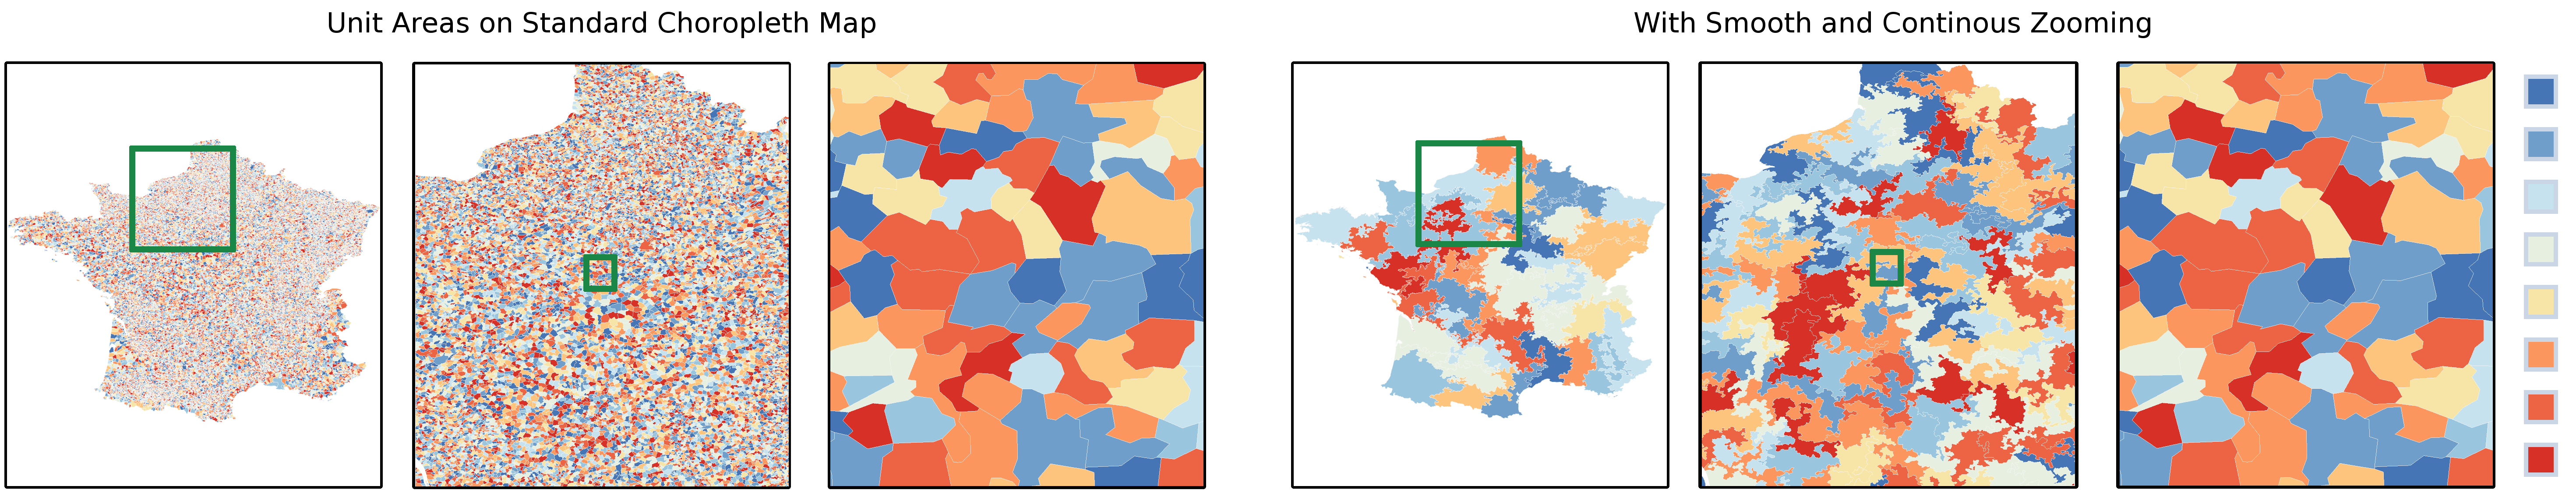
\includegraphics[width=\linewidth]{images/newTeaser}
  \caption{A comparison between a shape file representing France with over 30,000 administrative units and 729,565 vertices before and after the implementation of smooth zooming at 3 different levels of zoom, with minimum required screen space ($m$) of 1\%. Mapped colors from colorbrewer color palette \cite{colorbrewer}.  } \vspace{-0.2cm}
	\label{fig:teaser3}
\end{figure*}

Learning that scale is such a prevalent unsolved problem in the information visualization domain, this thesis examines the creation of interaction techniques to synergize with zooming functionality. The topic our initial investigations lies with is one of geospatial visualization's oldest and most common technique, the choropleth map.

Choropleth maps can be defined as displays where data is aggregated using administrative units and normalized values \cite{meirelles2013design}. Choropleths are ubiquitous for conveying area-based data on a geospatial map because they are intuitive and preserve geospatial information. However, because they do not distort geospatial boundaries, areas may be too small to perceive any data (see Figure \ref{fig:teaser}). This is especially true in the context of zooming where an area may not even cover a full pixel. Area-based data is often too dense to perceive in capital city regions. Ward \textit{et al.} state, "\emph{A problem of choropleth maps is that the most interesting values are often concentrated in densely populated areas with small and barely visible polygons, and less interesting values are spread out over sparsely populated areas with large and visually dominating polygons}" \cite{ward2010interactive}.


We focus on maintaining perceivable areas without map distortions by developing an area-merge algorithm that provides a user-controlled parameter, $m$, to display area units or area unit clusters that meet a minimum screen-space requirement. Rao and Card define such an adjust operation as ``\textit{...change the amount of contents viewed within the focus area without changing the size of focus area}" \cite{rao1994table}. By introducing a hierarchical representation of the choropleth, we can update the display quickly and enable changes to the level of detail for the best visual experience. We call this a dynamic choropleth map. Our zooming is smooth and continuous. By this we mean there are no jumps, distortions, or disruptions during the zooming. The level of detail changes dynamically and interactively without distorting the geometry. Changes in zoom level must be smooth and not rely on distortion of the geo-space or any areas contained within.


%\newpage
Our contributions include:
\begin{itemize}
\item A novel algorithm to interactively zoom smoothly, providing appropriate and perceivable levels of detail for choropleth maps.
\item Providing a set of pseudo-code to enable reproducibility of the method.
\item The application of our algorithm to complex, real-world shapefiles including those with over 10,000 unit areas and over 4.5 million vertices.
\end{itemize}
To provide this functionality, challenges must be overcome including developing an algorithm that detects when unit areas become too small, joining boundaries, building an appropriate area hierarchy, and zooming dynamically and continuously whilst preserving the traditional choropleth properties.
%\begin{enumerate}
%\item \textbf{identify contiguous regions} - A contiguous region refers to a set of units that all have at least one related neighbor. By identifying these regions, it will enable us to merge units with precise topological preservation.
%\item \textbf{identify a merge candidate} - In order to find a merge candidate, we must find a couple of units that meet are merge requirements (see section \ref{neighbors}). 
%\item \textbf{identify the shared boundary} - By identifying the shared boundary, we can create a clustered boundary that perfectly preserves the topological identity of both units from those of others. There are many challenges with identifying this shared boundary which can be found in section \ref{boundaryTree}.
%\end{enumerate}

In Section \ref{sec:relatedWork}, we review previous work on interactive zooming and choropleth maps. Section \ref{methodology} discusses the proposed methodology of the algorithm, a general overview of the procedure and the individual steps required. Section \ref{performance} discusses results and performance including benefits and limitations. 
%Section \ref{cfw} looks at potential future work and conclusions.

\begin{figure*}[t]
\centering
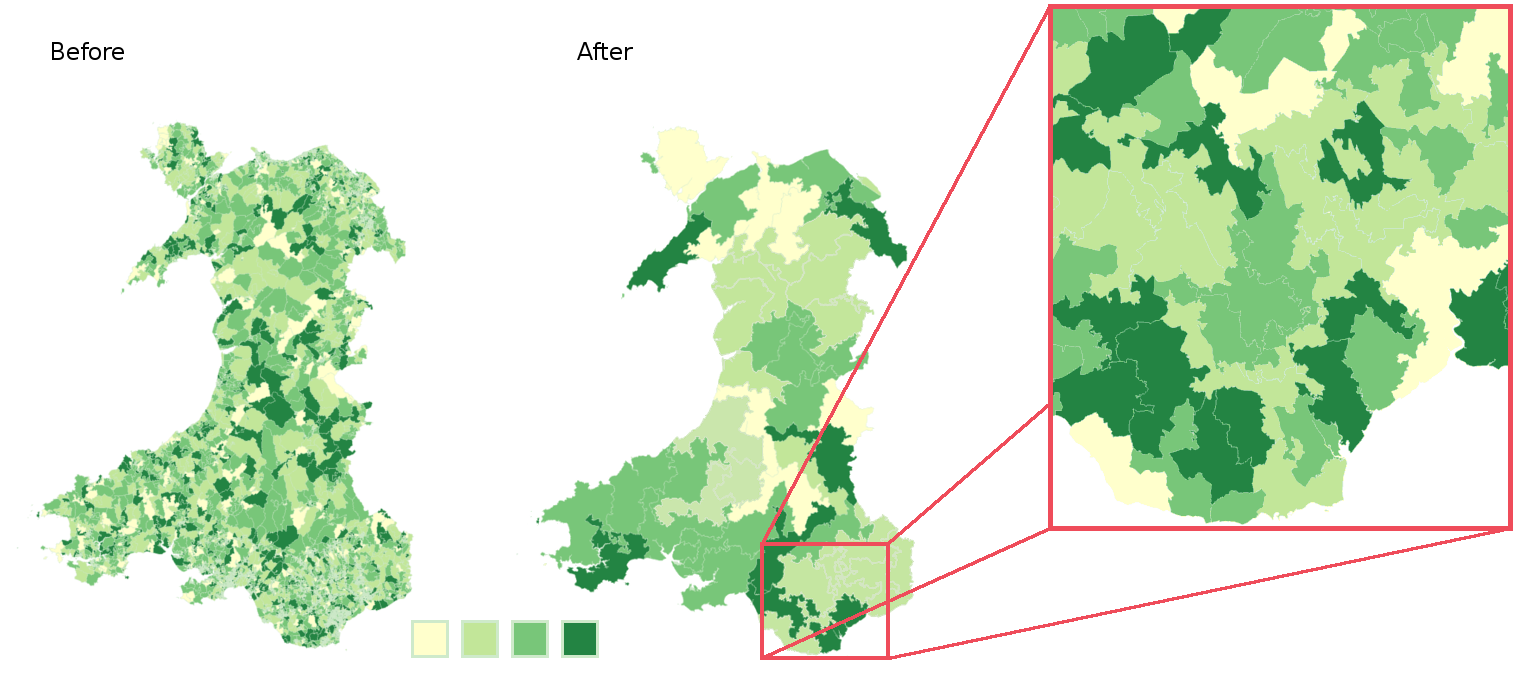
\includegraphics[width=1\linewidth]{images/Zooming3}
\caption{Example of the procedure applied to Wales \cite{wales}. The left image shows the original image with over 10,000 output areas having $4,652,800$ vertices \cite{vickers2007creating}, where we can see a dense clutter of indistinguishable areas in the south-east section. The right images shows the effects of the procedure at two different zoom levels (indicated by the red box), where $m$ is 2\%. Areas are color-mapped using colorbrewer color palette \cite{colorbrewer}. } \label{fig:zoomingExample} \vspace{0.2cm}
\end{figure*}


\section{Terminology}
Before we move any further, we provide a short guide on some important terminology related to our work.
\begin{table}[h]
\footnotesize
\begin{tabularx}{\textwidth}{ r | X }
Term & Definition\\ \hline \hline
Aggregation &  Aggregation is a grouping of similar information grouped in the form of an abstracted form. It is used to simplify complex definitions. \cite{slocum2009thematic} \\
Amalgamation & "the process of fusing nearby polygons" \cite{slocum2009thematic}. This can be used to amalgamate contiguous and non-contiguous regions and is a more detailed view than aggregation. In our case, we limit this to contiguous regions only. \\
Hierarchical agglomerative clustering & "Methods of cluster analysis that begin with each individual in a separate cluster and then, in a series of steps, combine individuals and later, clusters, into new, larger clusters until a final stage is reached where all individuals are members of a single group" \cite{everitt2006cambridge}. Our algorithm falls into this category.\\
Linkage & Linkage is a technique related to hierarchical agglomerative clustering depicting how clusters are selected for agglomeration. A few examples of this are single-linkage, which identifies the least distance between clusters, complete linkage which looks for the largest distance between clusters, and average linkage, which identifies the average distance between clusters \cite{everitt_2011}. Our algorithm leans towards Average linkage. \\
Dendrograms & A dendrogram refers to "a ‘tree-like’ diagram illustrating the series of steps taken by the method in proceeding from $n$ single member ‘clusters’ to a single group containing all $n$ individuals" \cite{everitt2006cambridge}. An example is provided in Figure \ref{fig:display}. \\
Graph-cut & A graph cut is the division of a set of graph nodes into two groups using a `cut'. An example of this can be found in Figure \ref{fig:display}.\\
Bottom-up & In this instance, bottom-up refers to how the data structure is created. As we are given a set of default areas to work with, we combine them until we hit the top of the data structure (1 area instance). Therefore we consider our approach bottom-up. \\
\hline \hline
\end{tabularx}
\caption{Terminology table.}
\end{table}


\section{Background} \label{sec:relatedWork}
The Survey of Surveys for information visualization, found in Chapter \ref{chap:SoS}, identifies one related survey paper on clutter reduction  \cite{ellis2007taxonomy}, no related surveys on the topic of choropleths or surveys focused on geo-spatial zooming, and one survey focused on hierarchical aggregation \cite{elmqvist2010hierarchical}. Ellis and Dix provide a taxonomy of clutter reduction for information visualization and review 11 clutter reduction techniques including clustering, space-filling, and animation  \cite{ellis2007taxonomy}.

\subsection{Zooming}
Cockburn \textit{et al.} review pan+zoom used in over 15 research papers, and examine overview+detail, zoom, and focus+context \cite{cockburn2008review}.
Rao and Card discuss the use of zooming for tabular information in the context of interactive manipulation of focus (zoom, adjust, and slide) \cite{rao1994table}. We require that the view and geometry are not distorted in any way in our work. Jog and Shneiderman present the zoom bar and introduce a zooming approach based on zooming towards a fixed-line within a starfield visualization \cite{jog1995starfield}. This differs from our work that focuses on choropleths. Van Wijk and Nuij provide an algorithm for smooth and efficient zooming across 2D planes \cite{van2003smooth} and extend on this idea by looking at non-uniform scaling between two planes \cite{van2004model}. They derive an optimal camera path for smooth zooming and panning. This is likely the previous work most similar to ours. Their work does not consider regions that may be too small to perceive which differs from our work. Also, the choropleth map is dynamic in our case. Javed \textit{et al.} present a zooming technique titled PolyZoom where a user progressively builds a hierarchy of focus regions to zoom between \cite{javed2012polyzoom}. Polyzoom focuses on different scales of maps separately whereas we endeavor to provide a continuous zooming method. Axelsson \textit{et al.} tackle challenges addressing visualization between large scales of information for astronomical data using scale scene graphs \cite{axelsson2017dynamic} which differs from our work that focuses on a single scene that must be smooth and continuous. Google Maps provides a map of the earth which enables the user to zoom on user-selected areas. Moving between zooming levels comes with sudden, discontinuous transitions between levels of detail which we avoid \cite{googleMaps}. Both Akelsson \textit{et al.} and Google Maps process image data broken up into rectangular tiles. Our algorithm processes original unit areas and handles geospatial boundaries composed of vertices and edges.

Blanch and Lecolinet provide zoomable treemaps that pan and snap-zoom between different levels within a treemap \cite{blanch2007browsing}. Roberts \textit{et al.} extend Van Wijk and Nuij's zooming work applying their smooth zooming algorithm to treemaps, and combine this with a smooth transition between levels of detail \cite{roberts2016interactive}. Our work differs from Roberts \textit{et al.} as our approach maintains a smooth and continuous transition between zoom levels, and selects what to display based the zoom level and a user-specified parameter. In addition, our work handles much more complex area-unit boundaries because it processes choropleths.


\subsection{Choropleths}
Digital choropleth maps have been produced prior to  1970 with the U.S Department of Commerce citing 10 choropleth mapping systems \cite{us1970use}. From our related work literature search, we find previous work on choropleths focus on class intervals (or systems) rather than zooming. A class is defined as a mutually exclusive and non-overlapping set of grouped data whilst a class interval is defined as the selected width (or range of data) of each class \cite{hooda1994statistics}. Tobler questions the use of class intervals within choropleth maps by reviewing the use of inked area vs. white area to display values \cite{tobler1973choropleth}. Brewer and Pickle provide a qualitative study on class intervals for choropleth maps comparing seven different methods \cite{brewer2002evaluation}. Zhang and Maciejewski detect critical boundary cases within choropleth maps where statistical measures fall near the selected classification bounds \cite{zhang2017quantifying}. This informs them of optimal selection of class intervals for data representation. Pickle presents a guideline for map design including color selection, legend design and smooth transition between color within area-units \cite{pickle2003usability}. Slocum \textit{et al.} provide a full chapter on Choropleth Mapping which includes 58 references \cite{slocum2009thematic} spanning 1957 \cite{stevens1957ratio} to 2006 \cite{anselin2006geoda}. They discuss decision-making behind classed and un-classed maps, appropriate color schemes, and designing the legend of the map \cite{slocum2009thematic}. Dykes and Brunsdon introduce new techniques for geographically weighted visualization using scalograms \cite{dykes2007geographically}. Each of these papers places emphasis on class intervals, whilst our chapter focuses on perceivable individual areas on a dynamic map.

Andrienko and Andrienko briefly survey the overall spatial distribution of data with diverging color scales in choropleth maps and provide an example of animated choropleth map displays with small multiples \cite{andrienko2006exploratory}. We do not review color scales or the use of temporal data in choropleth maps. 

Jern \textit{et al.} use linked views to observe regional development data using both a choropleth map and treemap \cite{jern2009treemaps}. Our chapter focuses on adding a new dynamic feature to choropleth maps rather than combining them with other techniques. Dang \textit{et al.} present a generalized map-based information tool for dynamic queries and brushing on choropleth maps \cite{dang2001dynamic}. Our work focuses on zooming rather than brushing. Li and Han look at applying the Lorenz curve to choropleth mapping to identify numerical trends \cite{li2010discovery}. We focus on user perceivability rather than new trends in data. Johansson \textit{et al.} present a web-based visualization tool that combines the use of choropleth maps with dashboard functionality in order to review multifaceted information on climate change and adaption measures \cite{johansson2017visadapt}. We focus on perceivability of unit areas, rather than the use of a choropleth map for climate change data. Speckmann and Verbeek present necklace maps which present choropleth maps with juxtaposed proportional symbol maps that allow the user to understand size data without distorting the topological view \cite{speckmann2010necklace}. We develop interactive, smooth zooming in order to address similar issues.

Rittschof and Kulhavy present a user-study which includes a comparison of choropleth maps and cartograms. Cartograms are a different class of related work considering a wide range of techniques (Gastner-Newman \cite{gastner2004diffusion}, Dorling \cite{dorling1993computer}, etc.) which use distortion to convey data. We want to avoid introducing geospatial error into the map in our technique. Their results found choropleth maps were associated with the greater recall of information \cite{rittschof1998learning}. Kasper reviews the effectiveness of Gastner-Newman diffusion cartograms \cite{kaspar2011empirical, gastner2004diffusion} for the representation of population data, which includes a comparative experiment against thematic maps (choropleth with overlayed circle maps). The results report that the thematic maps are more efficient and effective, specifically with complex tasks \cite{kaspar2011empirical}.
 Sun and Li review the effectiveness of cartograms for the representation of spatial data, which includes a comparative experiment against thematic maps including choropleths. The results indicate that the thematic maps are more effective representing quantitative data, whilst cartograms were more effective with qualitative data \cite{sun2010effectiveness}.
 
 To the best of our knowledge, no previous work focuses on dynamic and continuous zooming of choropleth maps while maintaining perceivable area units without distortion.
 
\subsection{Cartographic Generalization}
Slocum \textit{et al.} provide a full chapter on Cartographic scale and generalization \cite{slocum2009thematic}. The chapter defines generalization as: \textit{``the process of reducing the information content of maps because of scale change, map purpose, intended audience, and/or technical constraints"}, and reviews models of generalization include the models of Robin \textit{et al.} \cite{robinson1978elements} and McMaster and Shea \cite{mcmaster1992generalization}. Slocum \textit{et al.} define the fundamental operations of generalization as simplification, smoothing, aggregation, amalgamation, collapse, merging, refinement, exaggeration, enhancement, and displacement. Our algorithm uses recursive amalgamation on a per-area basis.

Elmqvist and Fekete provide a survey on hierarchical aggregation for information visualization \cite{elmqvist2010hierarchical}. The survey only provides one spatial aggregation techniques by Andrienko and Andrienko (discussed below). Andrienko and Andrienko briefly discuss aggregation with earthquake occurrences in Turkey \cite{andrienko2006exploratory}. They use a density map to aggregate the occurrences per rectangular grid cell. Andrienko and Andrienko's generalization approach looks at point data, whilst we focus on areas. Zhang \textit{et al.} present a novel visualization technique titled 'TopoGroups' \cite{zhang2017topogroups} used to group spatial data into hierarchical clusters to minimize visual clutter. Boundaries are used to present data topics as a stippled line, where the ratio of a stipple represents that of the data. We focus on polygon unification rather than point data.

Regnauld and Revell discuss their automatic amalgamation method used in producing the ordnance survey's scale maps \cite{regnauld2007automatic}. The paper uses several generalization techniques to select clusters (triangulation, proximity, and edge filtering) and manipulate the clusters to give a visually clear representation of amalgamated buildings. Our chapter looks at areas rather than buildings and is used for only contiguous areas. Li \textit{et al.} review amalgamation of buildings based on the Gestalt principles of design \cite{li2004automated} which include separation, length, and area thresholds as well as similarities in shape, size, and orientation. Our amalgamation technique does not allow for any separation and unites two areas instead. 

\section{Methodology} \label{methodology}
We begin with an overview of our methodology before discussing each step in detail. The algorithm is based on the premise that each area, starting with the unit areas, can be merged with its closest neighbor from smallest to largest to create a smooth and continuous transition for perceptible areas.

\subsection{Method Overview} \label{overview}

\begin{figure*}[t] 
\centering
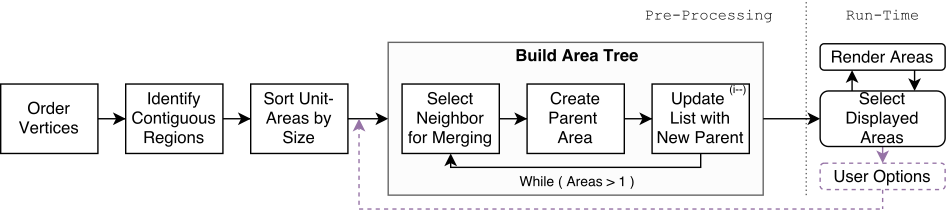
\includegraphics[width=1\textwidth]{images/HorizontalFlow2}
\caption{ The pipeline for the area amalgamation algorithm. After loading the shapefile, polygons are partitioned based on area contiguity, and sorted within islands (or land masses) based on their size. A recursive function is then used to identify new parent areas and their boundaries until their are no remaining neighbors to merge. See section \ref{methodology} for details. } \label{fig:procedure} \vspace{-0.2cm}
\end{figure*}

In order to effectively enable smooth and continuous zooming at run-time, we use pre-processing. We build a hierarchical data structure using hierarchical agglomerative clustering before displaying the choropleth. For this, we have created a pre-processing pipeline shown in Figure \ref{fig:procedure}. We first load each unit area represented by a polygon, $p$. A polygon $p$ is a list of vertices: $p = \{v_0,\dots,v_n\}$. We then update the order of each unit area's list of vertices to ensure that they are in clockwise order. The next step is to identify contiguous regions. Here we separate contiguous regions into islands (or land masses) which enforces topological continuity. Once each contiguous region is identified, each unit-area within the same contiguous region is sorted by size since the scale is an important part of the algorithm. It is more efficient to sort before building the hierarchical data structure.

The hierarchy construction is a recursive algorithm broken down into three sub-routines. As the regions are pre-sorted from smallest to largest, we know the first area merge candidate ($p_1$) is at the front. We must then find the second merge candidate ($p_2$) by selecting one of $p_1$'s neighbors using a distance function. When we have found a merge pair ($p_1, p_2$) we identify both the shared ($b_{s}$) and non-shared ($b_{ns}$) boundary of each, and combine such that $p_1$ and $p_2$ unite using only their shared boundary to create a new area $P$. 
\begin{equation} \label{eq:P}
P = (p_1 \cup  p_2) - (p_1 \cap p_2) 
\end{equation}
This is stored as a parent in the hierarchical data structure. When this is done, we can then remove the $p_1$ and $p_2$ from the merge candidates list and insert the new parent $P$ into the list preserving sorted order (by size). When there are no remaining neighbor candidates, the hierarchy is complete. When this is done for each contiguous region, we have the necessary hierarchical data structures for smooth zooming and clustering. 

With the hierarchies built, display is relatively simple. By specifying a desired minimum screen space, $m$, using the current zoom level and comparing that to each tree node's size using a depth-first search (DFS) in the hierarchy, we can select the appropriate polygons to display. An example of the results can be found in Figures \ref{fig:teaser3} and \ref{fig:zoomingExample}.

\subsection{Order Area Polygon Vertices} \label{ordering}
Our first step is to order the original vertex data from the shape file. This is important in order to reduce complexities in later stages. It allows us to simplify the identification of and unification of boundaries ($p_1 \cup p_2$). For this we use the shoelace formula (also known as Gauss's Area Formula or Surveyor's Formula), which allows us to derive both the area (useful for later) and the orientation \cite{braden1986surveyor}.
\begin{equation}\label{eq:surveyor}
a = \frac{1}{2} \left | \sum_{i=1}^{n-1} x_iy_{i+1} + x_ny_1 - \sum_{i=1}^{n-1} x_{i+1}y_i - x_1y_n \right |
\end{equation} 

The notation $x$ and $y$ refer to the coordinates of each vertex and $n$ refers to the number of vertices in $p$. If we remove the absolute value, we can deduce that if the area is negative, the vertex list is counter-clockwise, and we can reverse the list order. Unit-area's with multiple contiguous regions are also split up to enforce topological continuity. We process these islands (or land masses) as individual areas. We must also test for uncommon inner rings or any other vertices related to the shape. These can be saved in a separate list to aid in rendering, however, these must also be searched during boundary processing, as a ring found in unit-areas is usually formed as a result of a fully surrounded unit-area. In our Wales example (Figure \ref{fig:zoomingExample}) we find 31 instances of inner rings out of 30,000 polygons.

\subsection{Identifying Adjacent Neighbors \& Contiguous Regions} \label{neighbors}
After ordering each unit area's vertex lists, we can identify the contiguous regions. This is important for us in order to prevent a merge of two islands. The most important consideration is identifying what is classified as a neighbor. We provide pseudo-code for this in Algorithm \ref{alg:isneighbor}.

\begin{algorithm}[h]
\footnotesize
\caption{- Are polygons neighbors?}
\emph{Input--}\\
$p_{1}: \text{polygon one}$\\
$p_{2}: \text{polygon two}$\

\begin{algorithmic}[1]
\Procedure{isNeighbor($p_{1},~p_{2})$}{}
\If {isOverlapping( p1.boundingBox(),\\ ~~~~~~~~~~~~~~~~~~~~~~~~~~~~~~~~~~p2.boundingBox() )}
\State{\textbf{return} commonVertices($ p_{1}, p_{2}$)}
\IfEnd
\State {\textbf{return} \textsc{false}}
\EndProcedure
\end{algorithmic}
\emph{Local Variables--}\\
$counter:$ number of matching vertices\\
$MIN = 2:$ minimum number of matching vertices required to be neighbors 
\begin{algorithmic}[1]
\Procedure{ commonVertices($ p_{1}, p_{2}$) }{}
\State{counter = 0}
\For {i = 0;~i $< p_{1}$.length();~i++}
\If {$p_2$.intersects($p_1[i]$)}%commonVertex($p_{1}[i]$, $p_{2}$)}
\State{counter++}
\If{counter $\geq MIN$}
\State{\textbf{return} \textsc{true}}
\IfEnd
\IfEnd
\ForEnd{i}
\State{\textbf{return} \textsc{false}}

\EndProcedure
\end{algorithmic} \label{alg:isneighbor}
~\\
\textbf{Desc: }\emph{Compares two polygons and tests for overlapping boundaries,\\ $p_1 \cap p_2$. Returns true if the minimum number of common vertices are found. }
\end{algorithm}



We first test $p_1$ and $p_2$'s bounding boxes for overlap. By comparing Axis Aligned Bounding Boxes (AABB's) which use the maximum and minimum values for each axis of the areas $p_1$ and $p_2$ \cite{ericson2004real}, we ensure the in-depth neighbor checking is applied to as few areas as possible.
  
\begin{algorithm}[h]
\footnotesize
\caption{Contiguous Regions}
\emph{Input--} $L_{p}: \text{non-empty list of polygons}$\\
\emph{Output--} $L_{islands}: \text{list of contiguous islands (or land masses)}$\\
\emph{Local Variables--}\\
\textit{island}: current island\\
\textit{neighborFound}: flag designating if neighbor is part of existing island

\begin{algorithmic}[1] 
\Procedure{identifyContiguousRegions($L_{p}$)}{}
\State{\textit{// For each polygon}}
\While {!$L_p$.isEmpty()} 
\State{\textit{// Assume Island}}
\State{\textit{island} = $L_p$.popFirst()}
\State{\textit{// For each island}}
\For {i = 0; j $< L_{islands}$.length();~i++}
\State{\textit{// For each polygon on each island}}
\For {j = 0; j $< L_{islands}$[i].length(); j++}
\If {$ isNeighbor(island,L_{islands}[i][j])$}
\State{\textit{neighborFound} = true}
\State{\textbf{break}}
\IfEnd
\ForEnd{j}
\If{\textit{neighborFound}}
\State{island.appendList($L_{islands}$[i])}
\State{$L_{islands}$.removeIslandAt(i)}
\State{i- -}
\IfEnd
\ForEnd{i}
\State{$L_{islands}$.append(island)}
\WhileEnd
\State{\textbf{return $L_{islands}$}}
\EndProcedure
\end{algorithmic} \label{alg:contiguous}

~\\
\textbf{Desc: }\emph{Partitions a list of non-contiguous polygons into separate contiguous regions such as islands and landmasses. A contiguous region has connected neighbors where no area is completely separated by water. }
\end{algorithm}


If $p_1$ and $p_2$'s AABB intersect, we test their vertex lists for common points, where common points are considered identical coordinates. Algorithm \ref{alg:isneighbor} uses a simpler approach where we assume that all points have a matching point in a neighbor's vertex list. If areas with long straight edges (like some US states) are used to define unit-areas, we find cases where we need to use a second test to identify whether a point intersects a boundary edge (examples of this include T-junctions). We define neighbors as two polygons with at least two unique common vertices. We do not consider one common vertex as a boundary edge. The start and end of a shared boundary $b_s$ must also be considered the end and start of a non-shared boundary $b_ns$ to enforce topological continuity of the unit areas. 

\begin{figure}
\centering
\subfloat{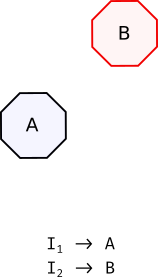
\includegraphics[width=0.2\textwidth]{images/Contiguous1}}~~~
\subfloat{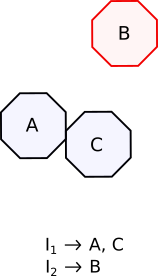
\includegraphics[width=0.2\textwidth]{images/Contiguous2}}~~~
\subfloat{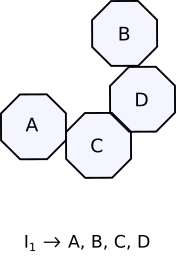
\includegraphics[width=0.2\textwidth]{images/Contiguous3}}~~~
\caption{ Visual example of the contiguous regions procedure. This shows how a potential contiguous region can be derived over three steps. See Section \ref{neighbors}.
} \label{fig:contiguousP} \vspace{-0.2cm}
\end{figure} 


Now that we can identify adjacent neighbors, we identify the contiguous regions. Pseudo-code is provided in Algorithm \ref{alg:contiguous}. We assume that our first unit-area is an island and test this against every other island. If an island contains a neighboring unit-area, we know that every other region on that island is also linked. Knowing this, we can merge the two polygon lists and continue our search. See Figure \ref{fig:contiguousP}. We must not finish the search here as our new unit-area may connect multiple islands. Once this is done for each unit-area, we have identified each contiguous region and each of these can be sorted based on their size. Figure \ref{fig:contiguousP} provides an example of the procedure, whilst Figure \ref{fig:contiguous} shows a visual result of this step.

\begin{figure}
\centering
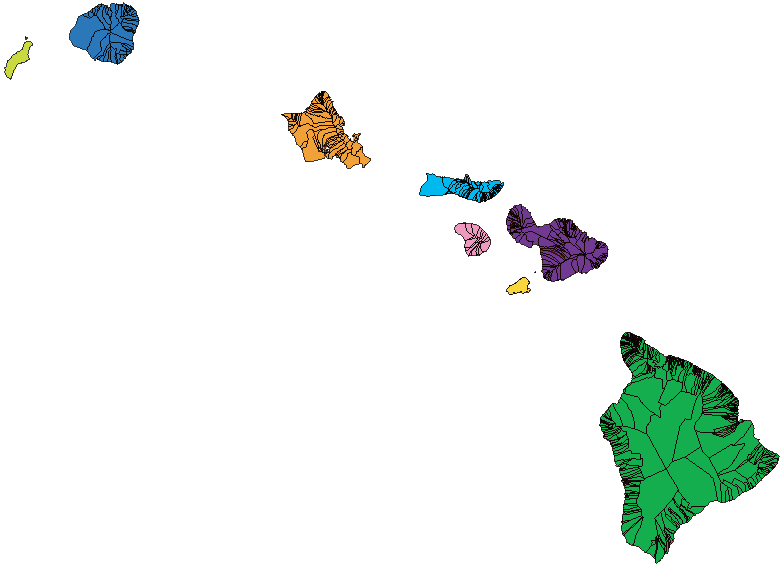
\includegraphics[width=.5\linewidth]{images/ahupuaa} 
\caption{Example of the contiguous regions procedure applied to the Ahupua'a boundaries of the state of Hawaii \cite{hawaii}. There are 10 visible contiguous islands each with their own color. See Section \ref{neighbors}.
} \label{fig:contiguous} \vspace{-0.2cm}
\end{figure}


\subsection{Building the Hierarchical Data Structure}
We use a recursive procedure to create a hierarchical data structure. A hierarchy is created for each contiguous region, where each area ($p_1$) is merged with it's closest neighbor ($p_2$). Distance is measured using a general and flexible metric described in Section \ref{boundaryTree}. We start with a merge candidate list filled with the sorted unit-areas (for one contiguous region). The list is sorted by size. As mentioned in Section \ref{overview}, there are three main sub-routines: neighbor selection, creating the parent area ($P$) and updating the merge candidate list. If only a single unit-area remains in the merge candidate list, no further merges can be processed and we have finished the procedure. Here we denote $p_1$ as the first area merge candidate, $p_2$ as the second merge candidate and parent $P$ (Equation \ref{eq:P}).

\subsection{Boundary Neighbor Selection \& Amalgamation Criteria} \label{boundaryTree}
%For neighbor selection, we select the smallest boundary neighbor merge candidate. We do this for a number of reasons. We search linearly through the list until we find a neighbor for $p_1$ and know this is the smallest as a result of the sorted list. Secondly, this allows us to simplify the algorithm. We can assume there is generally one $b_{s}$ between two neighbors. 
%%It becomes highly unlikely to find a configuration where two smaller unit area's surround a larger area. From our testing and research, we did not find any situation where this occurs.
%Other tested neighbor-selection types include selecting the closest center-point to $p_1$, or selecting the neighbor with the closest (or same) data value as $p_1$. We decided to design our procedure using the smallest neighbor selection as this choice aims to improve perceptibility. This matches our goal most closely.
In order to select an appropriate neighbor to join, we use a  general and flexible distance metric for amalgamation evaluated between neighboring areas. We use this to measure a distance where the closest distance is considered the optimal selection for a neighbor. The measure consists of four constituents: Smallest area ($a$), euclidean distance between centroids ($d$), value variance ($\alpha$), and shared boundary resolution ($b_s$). We formulate the measure as:

\begin{equation}
D = w_a.\frac{a}{a_{max}} + w_d.\frac{d}{d_{max}} + w_\alpha.\frac{\alpha}{\alpha_{max}} + w_{b_s}.(1-\frac{b_s}{b_{s_{max}}})
\end{equation}

The distance metric includes weight co-efficients which enable the user to customize the importance ($w$) of each criteria as an option, with a default weight 0.5 for $a$, and a $\frac{50}{3}$ weight for $d$, $\alpha$, and $b_s$.
We define the criteria as:
\begin{itemize}
\item Smallest area ($a$). The criterion tests the size of a neighbor. Searching for small areas is the primary objective of the procedure and it is therefore important to take this into account during the distance measure. By doing this we reduce the number of small areas at a faster rate. We discuss how the area is calculated in detail in Section \ref{ordering} (Equation \ref{eq:surveyor}). $a_{max}$ is considered the area of the canvas' bounding box.
\item Euclidean distance ($d$). This represents the shortest distance between the two centroids. By taking the distance between centroids into account, we can enable more natural polygon formations to form. To calculate this we can use ($\sqrt{(|p_1(c_x)-p_2(c_x)|)^2+(|p_1(c_y)-p_2(c_y)|)^2}$). The term $d_{max}$ is the largest distance between all centroids. 
\item Data Value Similarity ($\alpha$). Data is an important aspect of cartography and is considered when agglomerating areas. In order to factor it in the distance metric we look at the variance between the values of $p_1$ and $p_2$ ($|p_1(\alpha) - p_2(\alpha)|$). $\alpha_{max}$ is the largest data value in the data range.
%To calculate $n_{max}$, we use the largest distance between $p_1$'s value as well as minimum and maximum values of the dataset.
\item Shared Boundary Resolution ($b_s$). Unlike the other criterion, we favor a larger shared boundary resolution. The shared boundary resolution refers to the topological length of a shared boundary, where a larger shared boundary defines a closer unification between two areas. This is calculated by running our merge algorithms early (refer to Section \ref{parent} for more detail) and normalizing it over the largest resolution area in the tree ($b_{s_{max}})$. Once this is done, we subtract the normalized value from 1 to impose a stronger weight for larger shared boundaries.
\end{itemize}

Using these criteria, we can select an optimal amalgamation candidate. We also provide the user with the freedom to modify the criteria by using weighted coefficients. These can be modified after the procedure has been completed. This is a general and flexible distance metric because the distance metric itself is not a focus of the chapter. Many such metrics have been studied in great detail \cite{elmqvist2010hierarchical}. %However, the tree will need to be remodeled in order to replace any decisions the could be made at the merging process.

 \begin{figure}[p]
\centering
%\subfloat[Base Example]{
%\begin{tabularx}[1\textwidth]{CC} 
\scriptsize
\begin{tabularx}{1\linewidth}{c C}    
\multicolumn{2}{c}{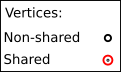
\includegraphics[width=0.15\linewidth]{images/caseLegend}} \\ \\

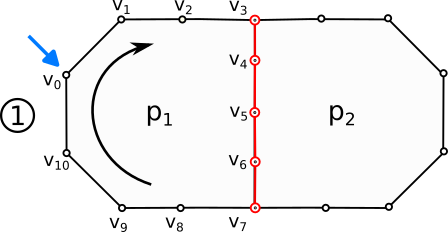
\includegraphics[width=0.3\linewidth, valign=m]{images/case1v2}  &$v_3-v_7$ form $b_{s}$ of $p_1$. $v_8-v_{10}$ and $v_0-v_2$ form $b_{ns}$ which is used to define the boundary of $p_1$ and $p_2$'s parent. \\ \\

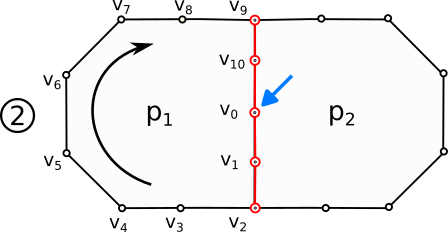
\includegraphics[width=0.3\linewidth, valign=m]{images/case2} &$v_0-v_2$ and $v_9-v_{10}$ are joined to form $b_{s}$ of $p_1$. $v_3-v_{8}$ form $b_{ns}$ which is used to define the boundary of $p_1$ and $p_2$'s parent. \\ \\

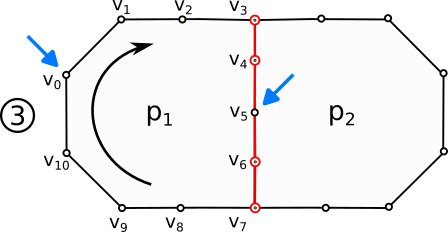
\includegraphics[width=0.3\linewidth, valign=m]{images/case5} &$v_3-v_4$ and $v_6-v_7$ form $b_{s}$ of $p_1$. $v_8-v_{10}$ and $v_0-v_2$ form $b_{ns}$ which is used to define the boundary of $p_1$ and $p_2$'s parent. $v_5$ is a vertex left by a previous merge from $p_1$'s children. This is considered a T-junction. \\ \\

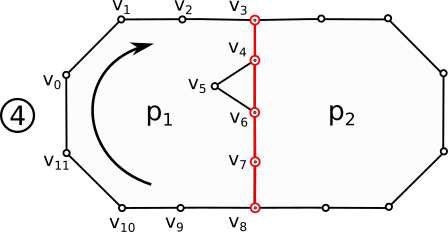
\includegraphics[width=0.3\linewidth, valign=m]{images/case3} &$v_3-v_4$  and $v_6-v_8$ form $b_{s}$ of $p_1$. $v_9-v_{11}$ and $v_0-v_2$ form $b_{ns}$ which is used to define the boundary of $p_1$ and $p_2$'s parent. $v_5$ is a vertex found within a $b_{s}$ and creates a void.\\ \\

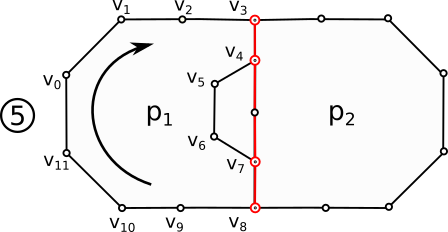
\includegraphics[width=0.3\linewidth, valign=m]{images/case4} &$v_3-v_4$ and $v_7-v_8$ form $b_{s}$ of $p_1$. $v_9-v_{11}$ and $v_0-v_2$ form $b_{ns}$ which is used to define the boundary of $p_1$ and $p_2$'s parent. $v_5-v_6$ is a $b_{ns}$ found within $b_{s}$ and can represent a river or a fissure between areas. \\ \\

\end{tabularx}   

%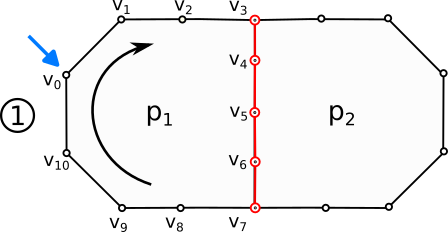
\includegraphics[width=0.3\textwidth]{images/case1v2}}& $V_3-V_7$ form the shared boundary of $P_1$. $V_8-V_{10}$ and $V_0-V_2$ are used to form the non-shared boundaries of $P_1$ and $P_2$'s parent boundary.\\

%\end{tabularx}
\caption{Different cases for $b_s$ and $b_{ns}$ identification. Case 1 displays the basic case where a whole boundary is found in contiguous order. Case 2 provides a contiguous order, but is split due to the location of $p_1$'s vertex list start index. Case 3 displays a T-junction which splits $b_{s}$ into two segments. This could be resolved by point-line intersection testing. Case 4 and 5 represent voids and fissures which cannot be resolved by point-line intersection, with the fissure having a possible size of $b_s.length-2$. We look at the length of common vertex chains to determine the start and end of $b_s$ detailed in Section \ref{parent}.
} \label{fig:boundary} \vspace{-0.3cm}
\end{figure}

\subsection{Creating Parent Area} \label{parent}
Creating $P$ includes 3 steps: (1) identify $b_{s}$ and $b_{ns}$ of each area's merge pair, (2) combining $b_{ns}$ of the $p_1$ and $p_2$ for the boundary of the parent area $P$, (3) linking $p_1$ and $p_2$ to $P$ for use in the rendering stage.

There are configurations which can cause unexpected challenges with boundary identification. Firstly, the vertex list of each area is ordered but there is no given information about shared boundaries. This means that $b_{s}$ can be found at any point within a vertex list, and can also start at any point with a vertex list. If our boundary search starts on $b_{ns}$ and we search the vertices in clockwise order, as in case 1 of Figure \ref{fig:boundary}, we can assume that the first common vertex is the boundary start. This is not the case for a first vertex found on $b_{s}$. In order to render the boundary correctly, we must not only identify $b_{s}$ but also identify the start and endpoints of the boundary. Figure \ref{fig:boundary} illustrates various cases identified for $b_{s}$ identification between two neighboring areas $p_1$ and $p_2$. 

Due to voids and fissures represented by rivers or other geographical features, finding the start and endpoints of $b_{s}$ can become complicated even when testing the entire vertex list. For example, if a vertex list begins on $b_{s}$ that includes a fissure of $n$ vertices, the selection of the $b_{s}$' beginning and end indexes becomes less obvious.

\begin{algorithm}[t]
\footnotesize
\caption{Identify Boundary Range}
\textit{Input--}\\
$start: \text{starting index of shared boundary line}$\\ 
$end: \text{last index of shared boundary line}$\\
$V_c: \text{current polygon vertices in clockwise order}$\\
$V_n: \text{neighbor polygon vertices in clockwise order}$\\
\textit{Local Variables--}\\
$longestC$: found by comparing  distance between common vertices\\
$common: \text{list of found commonVertices}$
\begin{algorithmic}[1]
\Procedure{identifyBoundaryRange($start, end, V_c, V_n$)}{}
\For{int i = 0; i < $V_c$.length(); ++i}
\If { $V_n$.contains($V_c$[i]) }
\State{common.append( $V_c$[i] )}
\IfEnd
\ForEnd{i}
\State{longestC = longestSharedBoundaryChain( common, $V_c$ )}
\State{*end = $V_c$.indexOf(common[longestC])}
\State{*start = $V_c$.indexOf(common[longestC.next()])}
\State {\textbf{return} }
\EndProcedure 
\end{algorithmic} \label{alg:sharedBoundary1}

~\\
\textbf{Desc: }\emph{Identifies $b_{s}$ for $V_c$ with $V_n$ as a neighbor. Required for parent node. }
\end{algorithm}
\begin{algorithm}[t]
\footnotesize
\caption{Longest Shared Boundary Chain}
\textit{Input--}\\
$common: \text{list of found commonVertices}$\\
$V_c: \text{current polygon vertices in clockwise order}$
\begin{algorithmic}[1]
\Procedure{LongestSharedBoundaryChain( common, $V_c$ )}{}
\If{ isLongestChain( $V_c$, $\&$longest, $V_c$.indexOf(common.last()),\\
~~~~~~~~~~~~~~~~~~~~~~~~~~~~~~~~~~~~~~$V_c$.indexOf(common.first()) )}
\State{longestIndex = common.length()-1}
\IfEnd
\For{i = 1; i < common.length(); i++}
\If{ isLongestChain( $V_c$, $\&$longest, $V_c$.indexOf(common.at(i-1)),\\
~~~~~~~~~~~~~~~~~~~~~~~~~~~~~~~~~~~~~~$V_c$.indexOf(common.at(i)) )}
\State{longestIndex = i}
\IfEnd
\ForEnd{i}
\State{\textbf{return} longestIndex}

\EndProcedure
\end{algorithmic}
\textit{New Input--}\\
$longestL$: The current longest distance between two common vertices\\
$currI$: current index to test\\
$nextI$: next index to test\\
\textit{Local Variables--}\\
$length$: length of current chain 
\begin{algorithmic}[1]
\Procedure{isLongestChain(V$_c$, longestL, currI, nextI)}{}
\State{ length = nextI - currI }
\If{ length < 0 }
\State{ length = length + current.size() - 1 }
\IfEnd
\If{ *longestL < length }
\State{*longestL = length}
\State{\textbf{return} true}
\Else
\State{\textbf{return} false}
\IfEnd
\EndProcedure
\end{algorithmic} \label{alg:sharedBoundary2}

~\\
\textbf{Desc: }\emph{Identifies the longest absence of a common vertex. We can assume that this signifies the beginning and end points of $b_{s}$. }
\end{algorithm}

 We provide our boundary identification process in Algorithm's \ref{alg:sharedBoundary1} and \ref{alg:sharedBoundary2} which identify the start and end vertices of $b_{s}$. 
Firstly, we search and identify every common vertex between the area neighbors. As discussed in Section \ref{neighbors}, we assume that every common vertex has a matching vertex in their neighbor's vertex list, whilst shapefiles with simpler boundaries may need an additional point to line intersection test (T-junctions). From these vertices we can identify the beginning and end indexes of $b_{s}$ (a common boundary between $p_1$ and $p_2$) by looking at the length of each common vertex chain. We use a heuristic that any voids and fissures found on $b_{s}$ will be smaller in length compared to $b_{ns}$ and therefore the longest chain between two common vertices signifies the chain between the end and the start of $b_{s}$. Figure \ref{fig:boundary} provides a visual presentation of boundary identification on some test cases encountered. This method handles cases with voids and fissures between neighboring polygons, as well as complications that can be caused by the T-junctions that may arise. For our Wales example in Figure \ref{fig:zoomingExample} with over 10,000 unit areas (over 20,000 merges) and 4.5 million vertices we found 11,112 individual error cases caused by voids, fissures, and T-junctions. This means a non-trivial case is found in over 55\% of the merges between $p_1$ and $p_2$.

Knowing $b_{s}$'s start and end indexes, we can easily separate the boundaries into $b_{s}$ and $b_{ns}$. We can then combine the $b_{ns}$ of an $p_1$ and $p_2$ in clockwise order to create the new parent area $P$. An example can be found in Figure \ref{fig:parent}.

\begin{figure}[t]
\centering
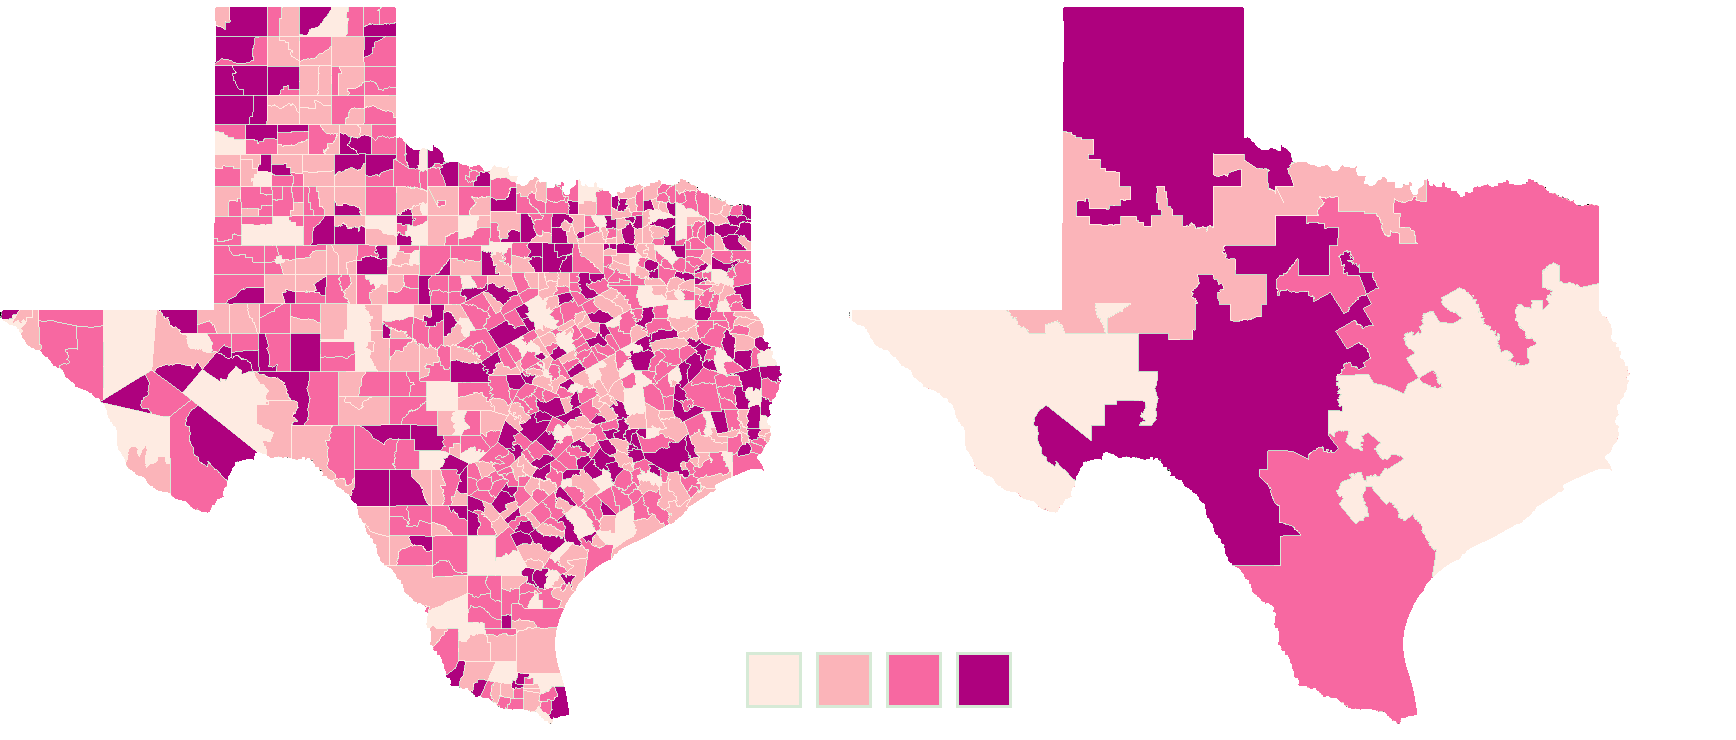
\includegraphics[width=0.7\linewidth]{images/TexasExample}
\caption{Example of derived parent area's from original unit-areas. The example uses the State of Texas and shows multiple boundary merges \cite{Texas} so that $m$ is 15\%.  See section \ref{parent}. Our example uses a color palette from colorbrewer \cite{colorbrewer}. } \label{fig:parent} 
\end{figure} 
 Once $P$'s vertex list is updated, we create pointers that enable $P$ to find it's children. This is important to enable traversal and selection within the hierarchical data structure. Algorithm's \ref{alg:sharedBoundary1} and \ref{alg:sharedBoundary2} detail this process.

\subsection{Updating the Sorted List with the Parent}
We update the list preserving the sorted areas. We first remove the $p_1$ and $p_2$ from our merge candidates list as each area can only be merged with one other area. Then we can insert $P$ into the list in sorted position based on its size. The procedure for building the hierarchical structure is found in Algorithm \ref{alg:binarytree}.

\begin{algorithm}
\footnotesize
\caption{Build Binary Tree}
\textit{Input--}\\
$L_{contig}: \text{contiguous list of polygon sorted by area}$\\
\textit{Local Variables--}\\
$neighborI:$ index of selected neighbor\\
$p:$ parent node of two neighbor areas
\begin{algorithmic}[1]
\Procedure{buildBinaryTree}{$L_{contig}$}
\If{$L_{contig}.length() > 1$}
\State{\textit{//Neighbor Selection}}
\State{neighborI = selectNeighbor(list) \textit{//neighbor of list.first()}}
\State{\textit{//Create Parent Area}}
\State{p = new Node()}
\State{p.identifyVertices($L_{contig}$.first(),$L_{contig}.at(neighborI)$))}
\State{p.setLeftChild($L_{contig}$.first())}
\State{p.setRightChild($L_{contig}$.at(neighborI))}
\State{$L_{contig}$.first().setParent(p)}
\State{$L_{contig}$.at(neighborI).setParent(p)}
\State{\textit{//Update Sorted List with Parent}}
\State{updateList($L_{contig},p,i$)}
\State{\textbf{return} buildBinaryTree($L_{contig}$)}
\IfEnd
\State{\textit{// Base Case -> $L_{contig} == 1$}}
\State{\textbf{return} $L_{contig}$}
\EndProcedure
\end{algorithmic} \label{alg:binarytree}

~\\
\textbf{Desc: }\emph{Builds hierarchy of polygons using a list of merge candidates recursively. }
\end{algorithm} 


\begin{figure}[ht]
\centering
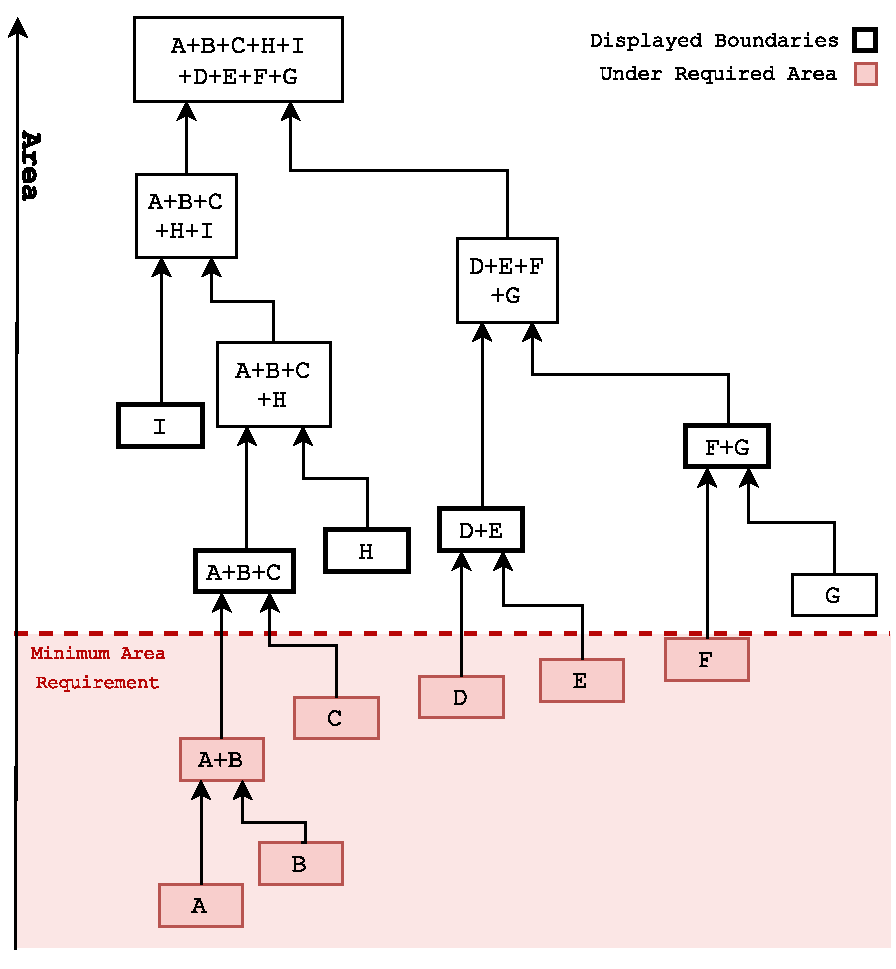
\includegraphics[width=0.7\linewidth]{images/displayBoundaries}
\caption{A dendogram depicting a typical hierarchical agglomerative cluster. An area is only rendered if one or both child nodes are smaller than the minimum area requirement, $m$. This is depicted by a graph cut. Otherwise, perform a depth-first search until  a leaf node is identified. In this example, \textbf{I, A+B+C, H, D+E,} \& \textbf{F+G} are selected to be rendered. See Section \ref{visible}. } \vspace{-0.2cm} \label{fig:display}
\end{figure}

\subsection{Selecting Visible Boundaries} \label{visible}
We select visible areas and boundaries based on a minimum area requirement, $m$, relative to the current screen space. As the screen space coverage changes based on the movement of the dynamic zoom level, we render different areas based on a zoom level and area size. The DFS identifies the smallest nodes in the tree that meet the minimum area size requirement. If any parent node is larger than the $m$, we test two criteria. (1) If the area is a leaf node, we can render the current node. (2) If either the left child or right child is smaller than $m$, then the current parent area is the smallest unit that meets the area requirement and is rendered. Completing the DFS will render only the smallest area within each branch that is larger than $m$. An illustrated example of this search can be found in Figure \ref{fig:display}. 

\subsection{Storing Values of Amalgamated Areas} \label{sec:value}
The Modifiable Areal Unit Problem (MAUP) \cite{openshaw1984modifiable} is an important aspect to consider when discussing the modification of boundaries or values. We address this by providing the user options to modify the calculation of aggregated values as well as the weighted distance metric discussed in Section \ref{boundaryTree}. The data is linked to the administrative areas during the initial loading of the shapefiles. Before the area tree is built, the user can select the type of value amalgamation. This enables the user to choose options of sums, qualitative frequencies, and averages.  When amalgamating values using sums, the value of $P$ can be calculated as $P(\alpha) = p_1(\alpha)+p_2(\alpha)$. Qualitative values are calculated using frequencies. Using a DFS, $P$ can count the frequency of each value for each leaf node and use the value of the most frequent of the leaf nodes. This is useful for categorical data. The average and weighted average  can also be calculated using a DFS, by calculating the sum, $P(\alpha) = \sum_{i=0}^{i=n} \frac{p_{\l  i}(\alpha)}{p_{\l i}(a)}$, where $p_{\l} $ denotes a leaf node in the tree. Examples are shown in Figure \ref{fig:valueCalc}.

\begin{figure*}[t]
\centering
\subfloat[Sum]{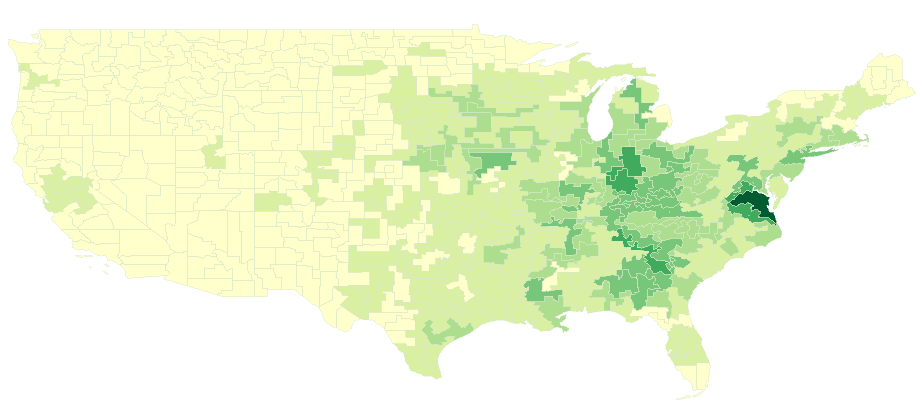
\includegraphics[width=0.8\linewidth]{images/sum}}\\
\subfloat[Frequency]{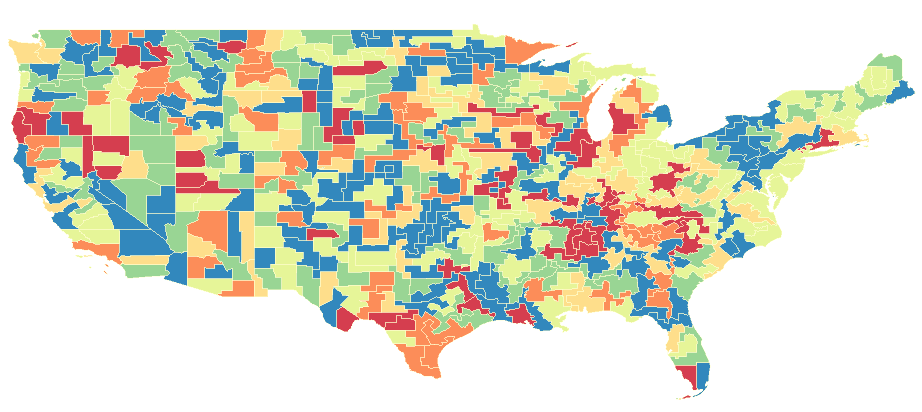
\includegraphics[width=0.8\linewidth]{images/frequency}}\\
\subfloat[Average]{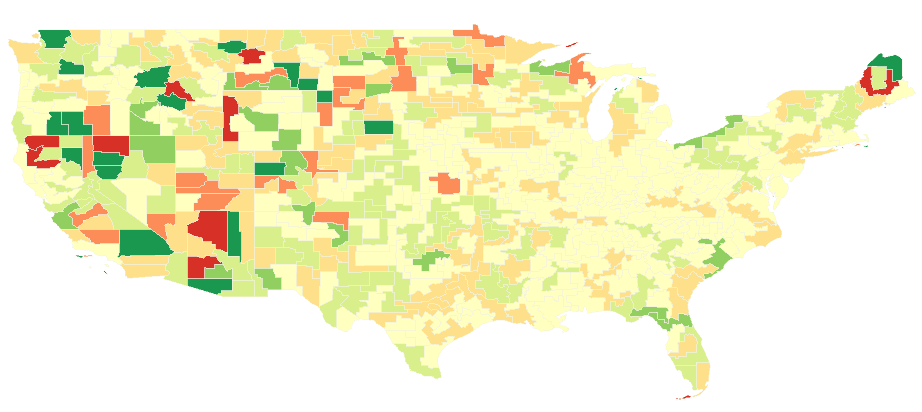
\includegraphics[width=0.8\linewidth]{images/average}}
\caption{ 1 value-set displayed using 3 different base-calculation types using US counties ($m$=0.3\%). (a) Represents using the sum to calculate the new values (sums). (b) Uses the highest frequency to represent values (qualitative data). (c) Uses the average of the value from all leaf nodes.  See Section \ref{sec:value}. } \label{fig:valueCalc} \vspace{-0.2cm}
\end{figure*}

As well as these value criteria, these can be normalized at the rendering stage. Some examples of these normalization techniques include area ($\frac{P(\alpha)}{P(a)}$), population ($\frac{P(\alpha)}{P(\kappa)}$), as well as any ratio ($\frac{P(\alpha)}{P(\delta)}$).

Although the normalization can be turned on and off after the area tree is built. In order to change value representations, the build area tree procedure is re-run.



%%%%%FULL TABLE%%%%%
%\begin{figure*}[t]
%\centering
%\subfloat[Table of Performance]{%\pgfplotstabletypeset[string type,
%%columns/area/.style={column name=Number of Unit-Areas},
%%columns/contiguous/.style={column name =  `Contiguous' Time (mm:ss)},
%%columns/merge/.style={column name= `Merge' Time (mm:ss)} ]
%%{data/performance.txt}
%\ra{1.5}
%\begin{tabularx}{1\linewidth}{@{}c c b{1.3cm} b{1.2cm} c C C C  c C@{}} \toprule 
%
%\multicolumn{1}{m{1.3cm}}{\centering \textbf{Shape File}} 
%&\multicolumn{1}{m{1.3cm}}{\centering \textbf{Number of Areas}} 
%&\multicolumn{1}{m{1.3cm}}{\centering \textbf{Total Vertices}} 
%&\multicolumn{1}{m{1.2cm}}{\centering \textbf{$\frac{\text{Vertices}}{\text{Area}}$}} &
%&\centering \textbf{Order Vertices (mm:ss.ms)}
%&\centering \textbf{Contiguous Regions (mm:ss)}
%&\centering \textbf{Build Hierarchy (mm:ss)} &
%& \textbf{Average FPS (5\% Screen space Threshold)}\\ 
%
%\cmidrule[0.4pt](r{0.5em}){1-1}
%\cmidrule[0.4pt](r{0.5em}){2-2}
%\cmidrule[0.4pt](r{0.5em}){3-3}
%\cmidrule[0.4pt](r{0.5em}){4-4}
%\cmidrule[0.4pt](r{0.5em}){6-6}
%\cmidrule[0.4pt](r{0.5em}){7-7}
%\cmidrule[0.4pt](r{0.5em}){8-8}
%\cmidrule[0.4pt](r{0.00em}){10-10}
%\rowcolor[gray]{0.925}
%\textbf{US Counties} &3,134 &\flushright 51,891 & \flushright 16.56 && 00:00.027 & 00:07 & 00:12 && 30.134 \\ 
%\textbf{Japan} &3,223 &\flushright 869,386 &\flushright 269.744 && 00:00.094 & 01:16& 01:57 && 6.234 \\ \rowcolor[gray]{0.925}
%\textbf{Italy} & 8,946 &\flushright 966,206 & \flushright 108.004&& 00:00.162 & 02:59 & 07:03 && 10.013\\ 
%\textbf{Wales} & 10,355&\flushright ~4,652,800 &\flushright 449.32&& 00:00.452 & 09:18 & 18:18 && 5.027\\ \rowcolor[gray]{0.925}
%\textbf{Germany} & 12,416 &\flushright ~1,934,800 &\flushright 155.779&& 00:00.293 & 10:24 & 32:10 && 6.451\\
%\bottomrule
%\end{tabularx}}
%\caption{%(a) 
%The results of performance. We present some attributes related to the shape file, performance times broken into seperate sections of the procedure, and the average FPS. The FPS is set to a minimum required screen space of 5\% for polygon rendering.
%% (b) The performance results as a bar graph.
%} \label{fig:performance}
%
%\end{figure*}

%\begin{figure}
%\addtocounter{subfigure}{1}
%\subfloat[Results Graph]{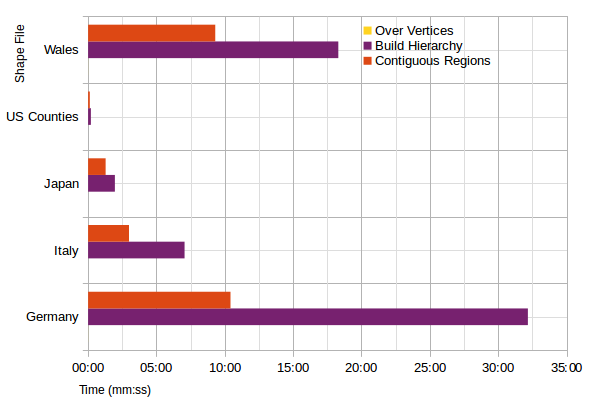
\includegraphics[width=1\linewidth]{data/graphNewA}}
%\caption{(a) The results of performance. We present some attributes related to the shape file, performance times broken into seperate sections of the procedure, and the average FPS. The FPS is set to a minimum required screen space of 5\% for polygon rendering. (b) The performance results as a bar graph.} \label{fig:performance}
%\end{figure}

\section{Results and Performance} \label{performance}
The desktop used to test this implementation features an Intel i5-4460 at 3.2GHz with 16GB of RAM and a GeForce GTX960. The implementation is developed using the Linux Mint 18 environment and the C++ framework of Qt. The software uses the Geospatial Data Abstraction Library to read the Shape File's unit-area information \cite{GDAL} and the OpenGL library to render the results.

%We test the algorithm based on a range of different shapefiles for performance. We add an in-line timer to capture the performance from the loading of the shapefile until all the data-structures have been stored and sent to the canvas.  The results can be found in Figure \ref{fig:performance}.

\begin{table}[t]
\centering \footnotesize
\subfloat{%\pgfplotstabletypeset[string type,
%columns/area/.style={column name=Number of Unit-Areas},
%columns/contiguous/.style={column name =  `Contiguous' Time (mm:ss)},
%columns/merge/.style={column name= `Merge' Time (mm:ss)} ]
%{data/performance.txt}
\ra{1.5}
\begin{tabularx}{0.6\linewidth}{@{}c c b{1.7cm} b{1.1cm} C@{}} \toprule 

\multicolumn{1}{m{1.3cm}}{\centering \textbf{Shape File}} 
&\multicolumn{1}{m{1.3cm}}{\centering \textbf{Number of Areas}} 
&\multicolumn{1}{m{1.7cm}}{\centering \textbf{Total Vertices}} 
&\multicolumn{1}{m{1.1cm}}{\centering \textbf{$\frac{\text{Vertices}}{\text{Area}}$}}
& \textbf{Average FPS,\newline $m$ = 5\%}\\ 

\cmidrule[0.4pt](r{0.5em}){1-1}
\cmidrule[0.4pt](r{0.5em}){2-2}
\cmidrule[0.4pt](r{0.5em}){3-3}
\cmidrule[0.4pt](r{0.5em}){4-4}
\cmidrule[0.4pt](r{0.00em}){5-5}
\rowcolor[gray]{0.925}
\textbf{US Counties} &3,134 &\flushright 51,891 & \flushright 16.56 & 30 \\ 
\textbf{Japan} &3,223 &\flushright 869,386 &\flushright 269.744 & 21 \\ \rowcolor[gray]{0.925}
\textbf{Italy} & 8,946 &\flushright 966,206 & \flushright 108.004 & 9\\ 
\textbf{Wales} & 10,355&\flushright ~4,652,800 &\flushright 449.32 & 5\\ \rowcolor[gray]{0.925}
\textbf{Germany} & 12,416 &\flushright ~1,934,800 &\flushright 155.779 & 6\\
\textbf{France} & 37,227 &\flushright 729,556 & \flushright 19.597 & 4\\
\bottomrule
\end{tabularx}}
\caption{%(a) 
The results of performance. We present some attributes of each shape file and the average FPS (frames per second). The FPS is set to a minimum required screen space of 5\% for polygon rendering.
% (b) The performance results as a bar graph.
\vspace{-0.2cm} }\label{fig:performance}

\end{table}

We test 5 different shapefiles of varying resolution including US Counties, Japan, Italy, Wales, and Germany found using the Global Administrative Areas website \cite{GAA}. There is a large variance in the number of areas, the average number of vertices, total contiguous regions, and coordinate space range. We know of no closely related previous algorithm that we can compare performance with. See Figures \ref{fig:teaser3} to \ref{fig:zoomout2} for results imagery. See the accompanying video for more dynamic results.

The performance is not only reliant on the number of unit areas but also the complexity of unit areas, and the total number of contiguous regions. A summary is found in Figure \ref{fig:performance}. Pre-processing can require a few minutes however it is only a one-time cost.
 
We found that different shapefiles for the same region would garner inconsistent topologies, which even includes the contiguity of the unit-areas. This makes it impossible to compare our fully merged areas to already existing shapefiles as a way of testing the topology-preserving nature of our implementation. 


%\section{Supplementary Material} \label{sec:sm}
%We include a variety of supplementary material including additional images, the referenced pseudo-code is also included to allow the user a more fundamental understanding of the procedures we discussed. This can be found at: \url{https://bit.ly/2GGCe6v}. Finally, we present a short video discussing the paper in an audio-visual format which can be found at: \url{https://bit.ly/2wYX0Ok}. For this paper, we use GADM, as well as United Stated Census Data \cite{GAA, USCB} to test our algorithm. In our video presentation, we use data to present the value calculation aspect of our algorithm found at the United Stated Census Data, and Office for National Statistics \cite{USCB2, ONS}.

%\section{Future Work \& Limitations} \label{cfw}
%There are many avenues for future work. Although we use real unit-areas, we would like to test with a wider range of choropleth data. The algorithm still has performance optimizations which could accelerate the speed even further, such as schematization \cite{barkowsky2000schematizing} which could be used to enable better optimization with topological continuity being reduced. Other existing formats such as TopoJSON \cite{bostock2018topojson} look at reducing geometry redundancy and could be a good subsequent format for the procedure. We can also continue with the idea of pre-processing by adding ways to improve performance on a second pass-through such as saving build instructions to reduce the calculation of neighbor and boundaries. We worked with 2D coordinate-spaces. A 3D coordinate space would be an interesting direction to take the algorithm and could open new applications. The current termination method revolves around the idea of one area per contiguous region. Updates in the procedure could allow for more user control when it comes to stopping the merge procedure such as for categorical data where the most abstraction is introduced. Alternatively to this, a bi-variate color map could be implemented to display more accurate concordance of underlying values.  The algorithm potentially can apply to any data-sets with geometric boundaries and is open to new data-structures. We can also test the usability by providing user studies on the minimum perceivable screen space using the algorithm. The use of this study could reach further than this visualization technique.

\section{Conclusion}
We introduce a novel method of smooth and continuous zooming by exploiting a hierarchical data structure to merge areas based on their sizes and shared boundary. The shared boundary is found by first comparing the vertex list of two neighboring areas and finding the longest vertex chain between common vertices. We then render only the perceivable areas or area clusters based on the current zoom level and screen space. This method of rendering improves perceptibility whilst still providing an understanding of the underlying data without distorting the map. This enables the user to zoom without any distortion to the geometry and enables clear perceivable choropleth data for the user. 

%\section{Acknowledgements}
%We would like to thank KESS for contributing funding towards this endeavor. Knowledge Economy Skills Scholarships (KESS) is a pan-Wales higher level skills initiative led by Bangor University on behalf of the HE sector in Wales. It is partially funded by the Welsh Government's European Social Fund (ESF) convergence programme for West Wales and the Valleys. We also thank GoFore UK for contributing funds to this endeavor. We thank Dylan Rees for proofreading the paper. We also thank Thomas Basketter for testing content comprehension. We thank Amy Mizen for giving us domain expert feedback and advice.

\begin{sidewaysfigure}[t]
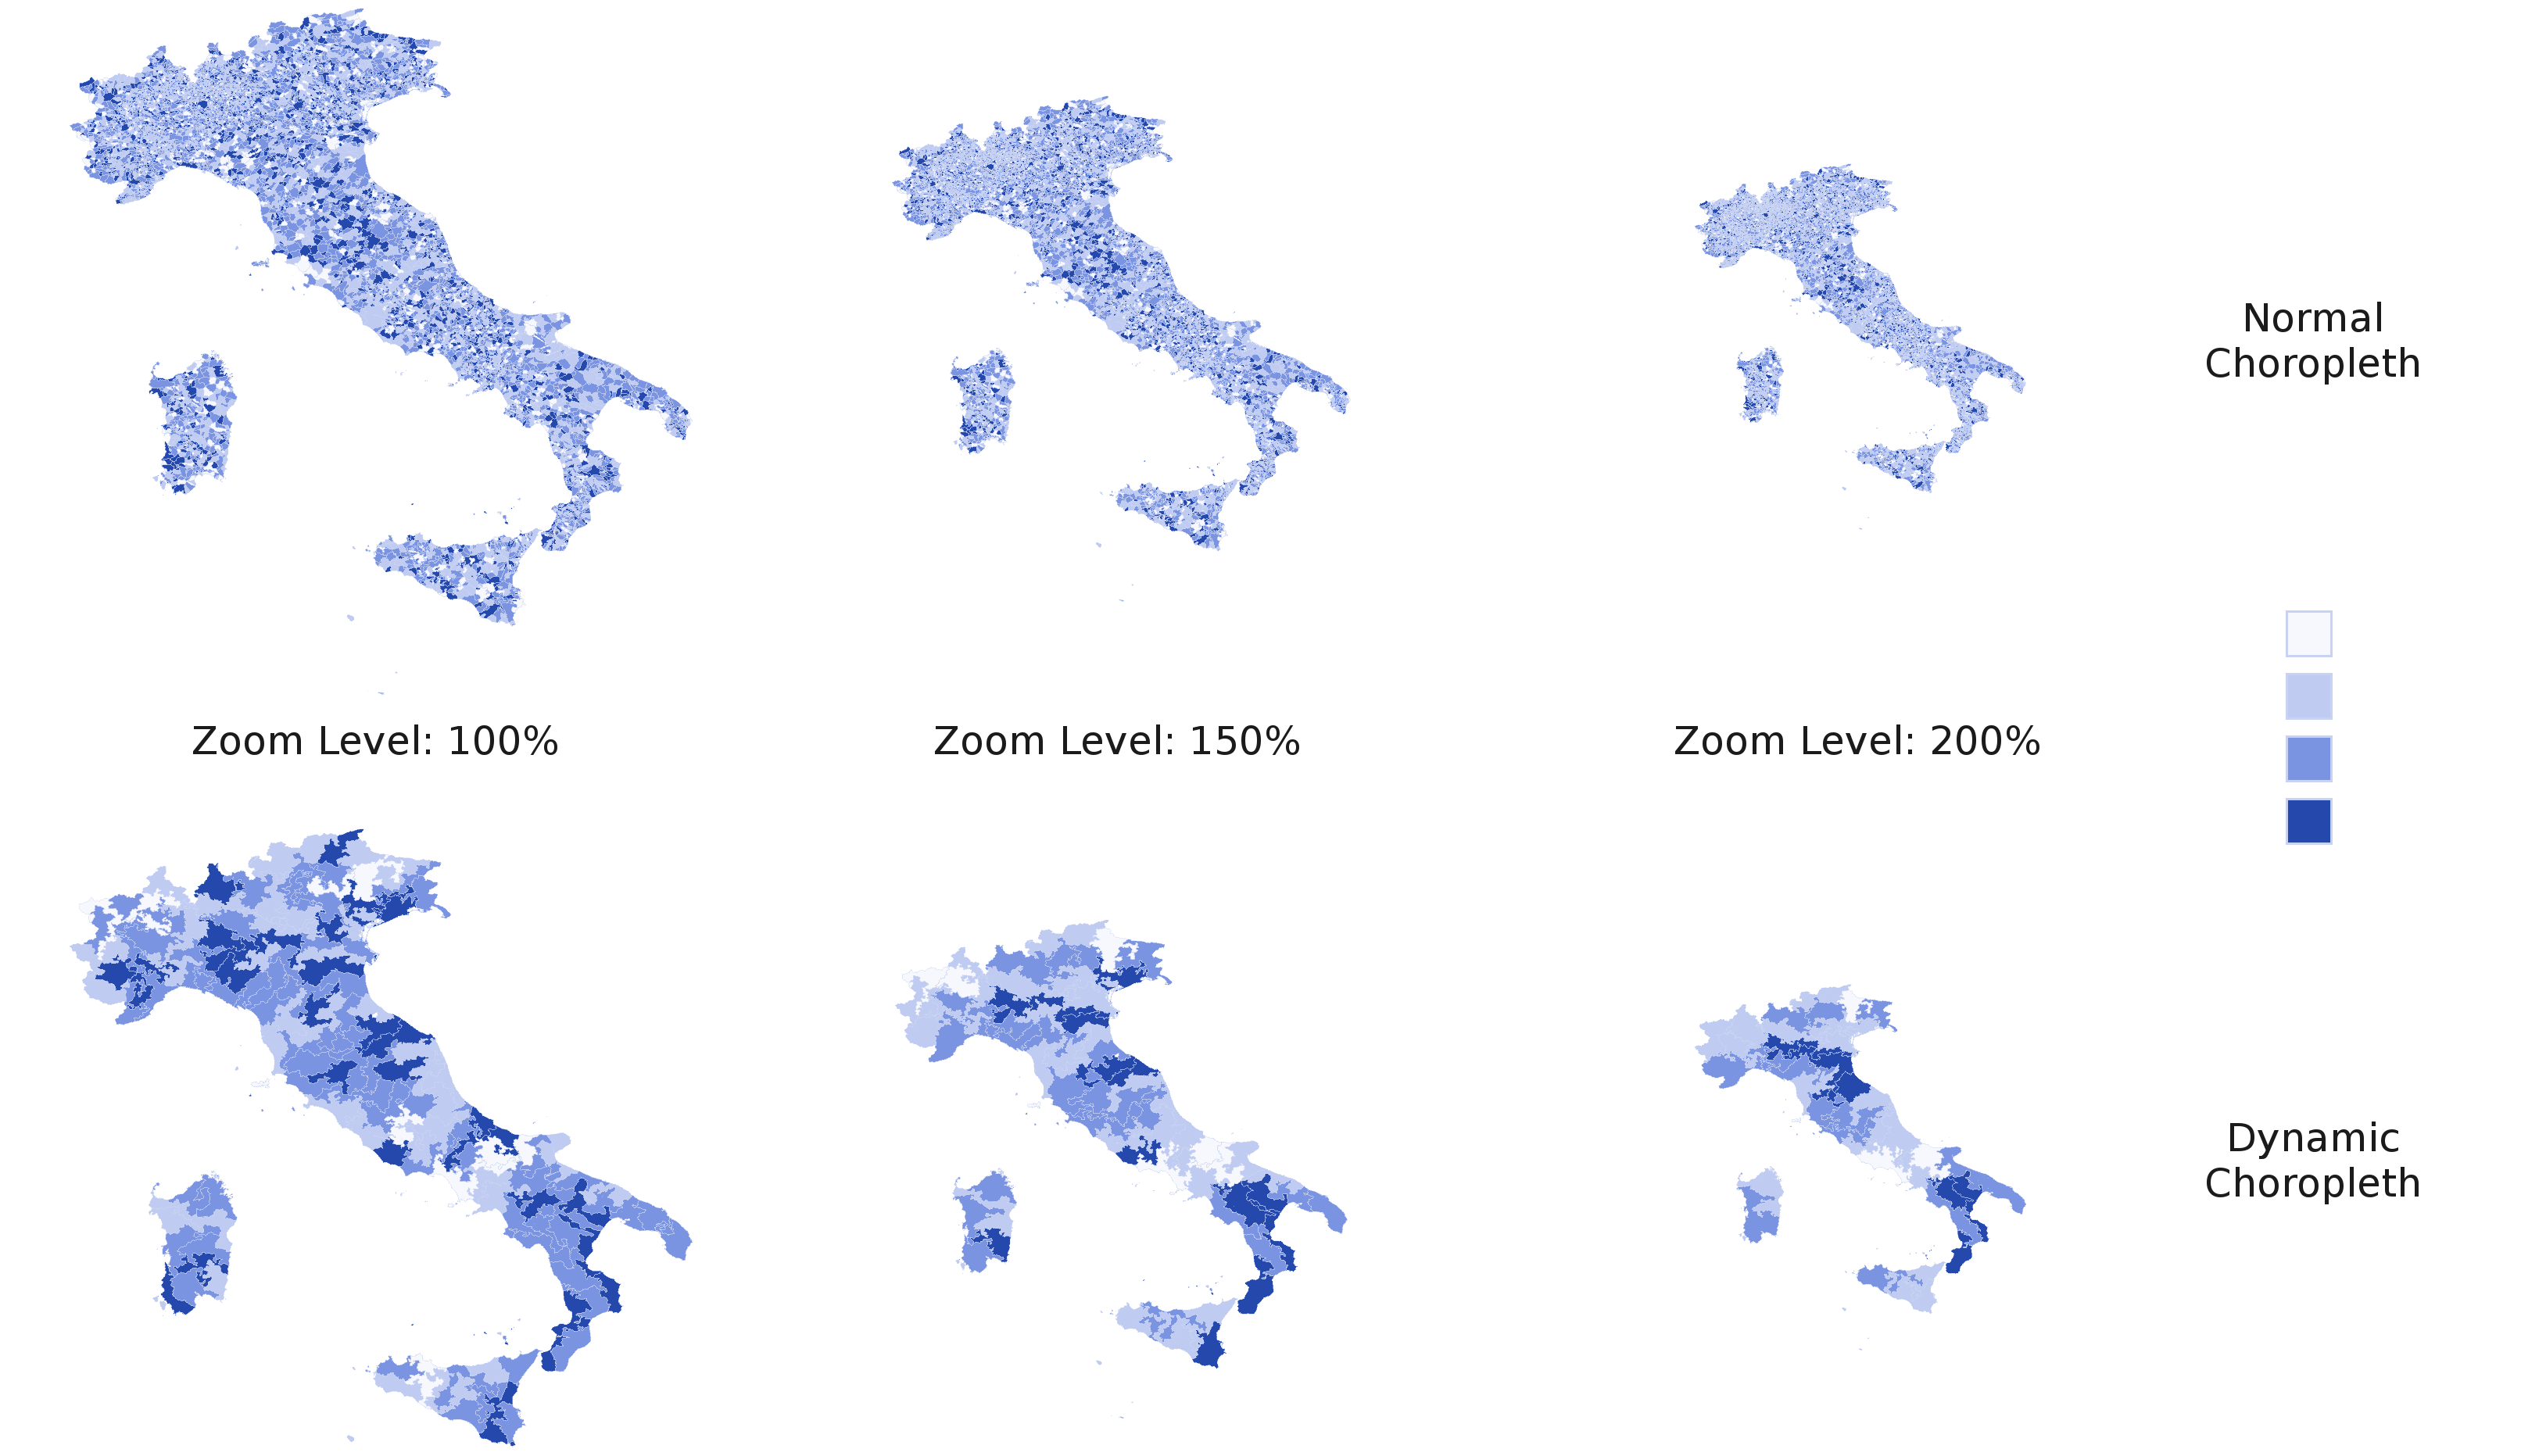
\includegraphics[width=1\linewidth]{images/zoomOutExample}
\caption{An example of zooming out of Italy's administrative units where $m$ = 1\%.} \label{fig:zoomout}
\end{sidewaysfigure}
\begin{sidewaysfigure}[t]
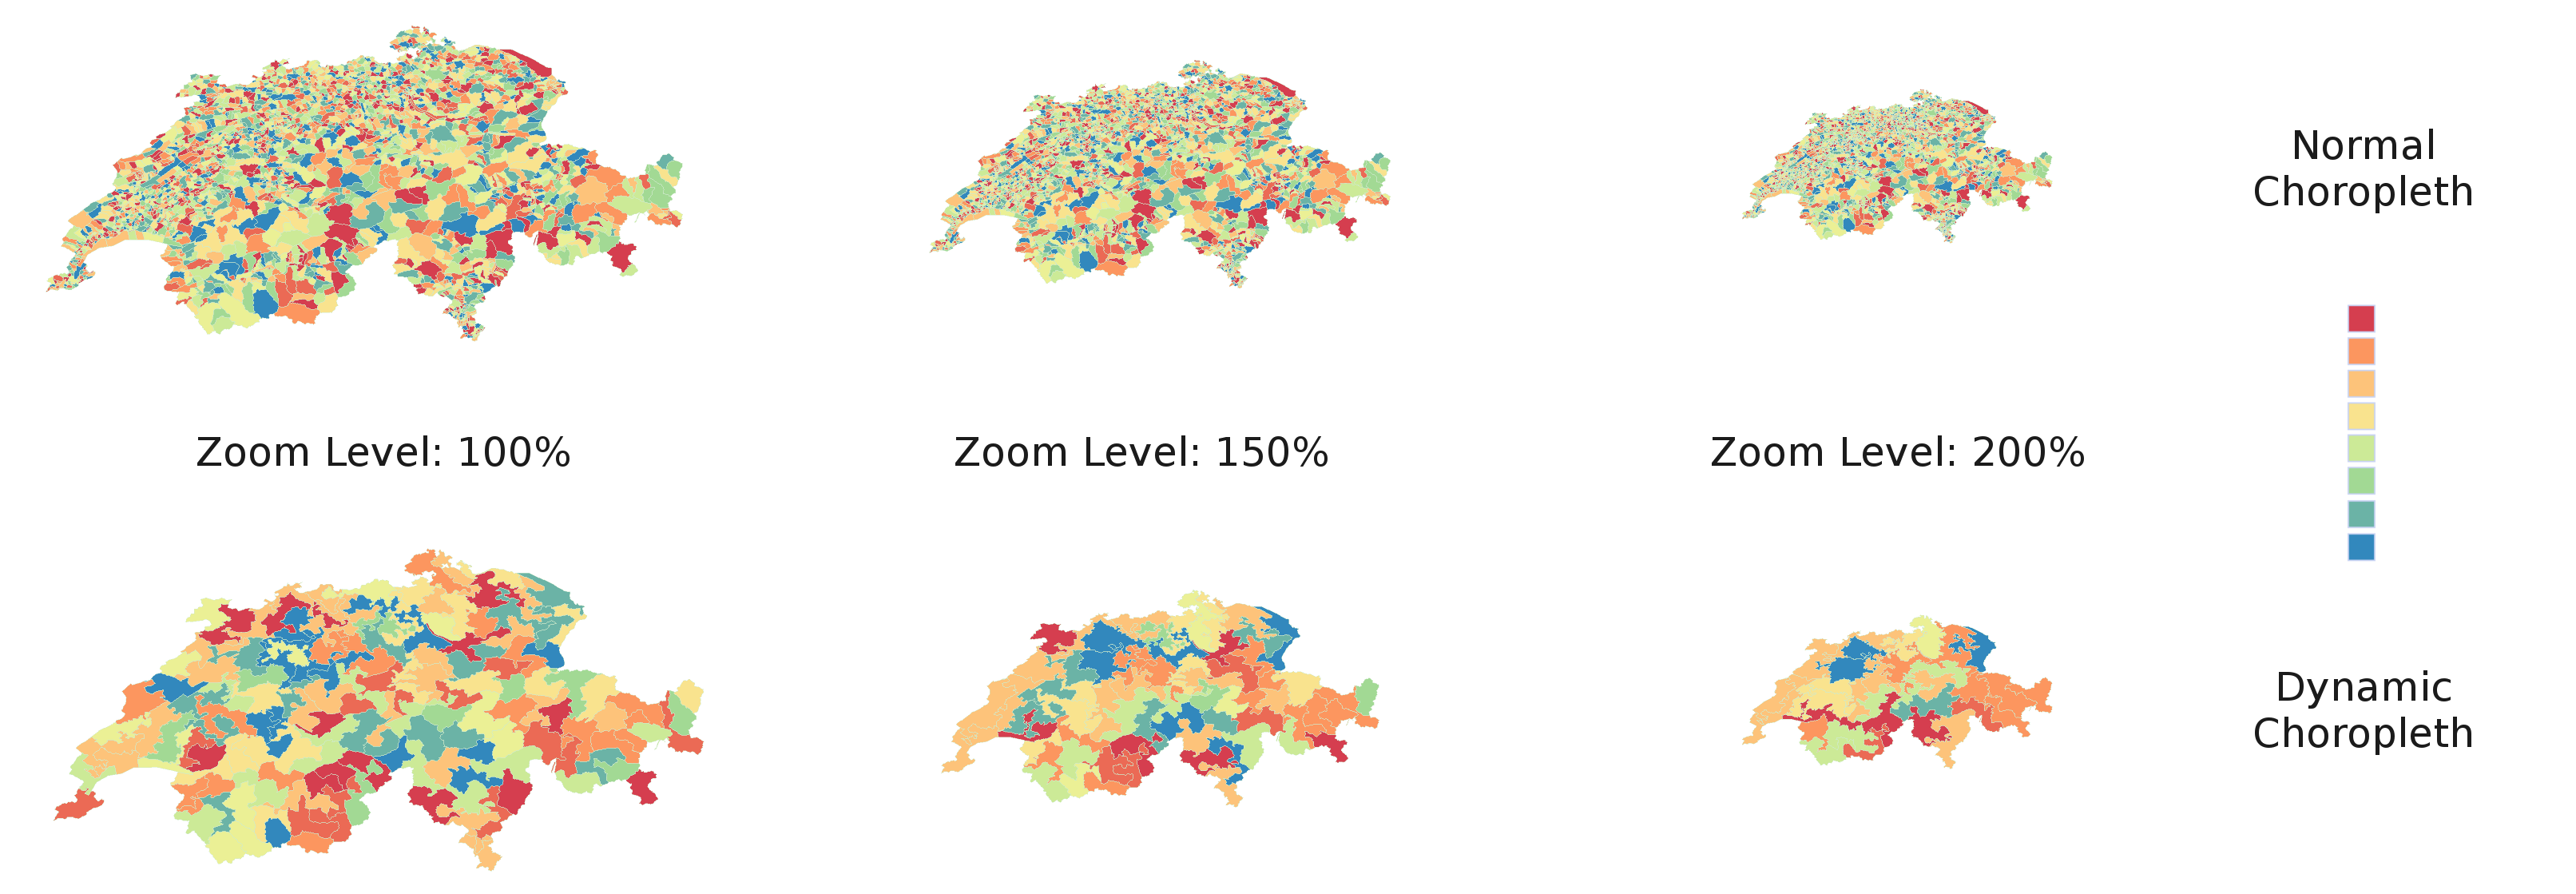
\includegraphics[width=1\linewidth]{images/zoomOutExample2}
\caption{ An example of zooming out of Switzerland's administrative units where $m$ = 1\%.}\label{fig:zoomout2}
\end{sidewaysfigure}

\begin{sidewaysfigure}[p]
\subfloat[]{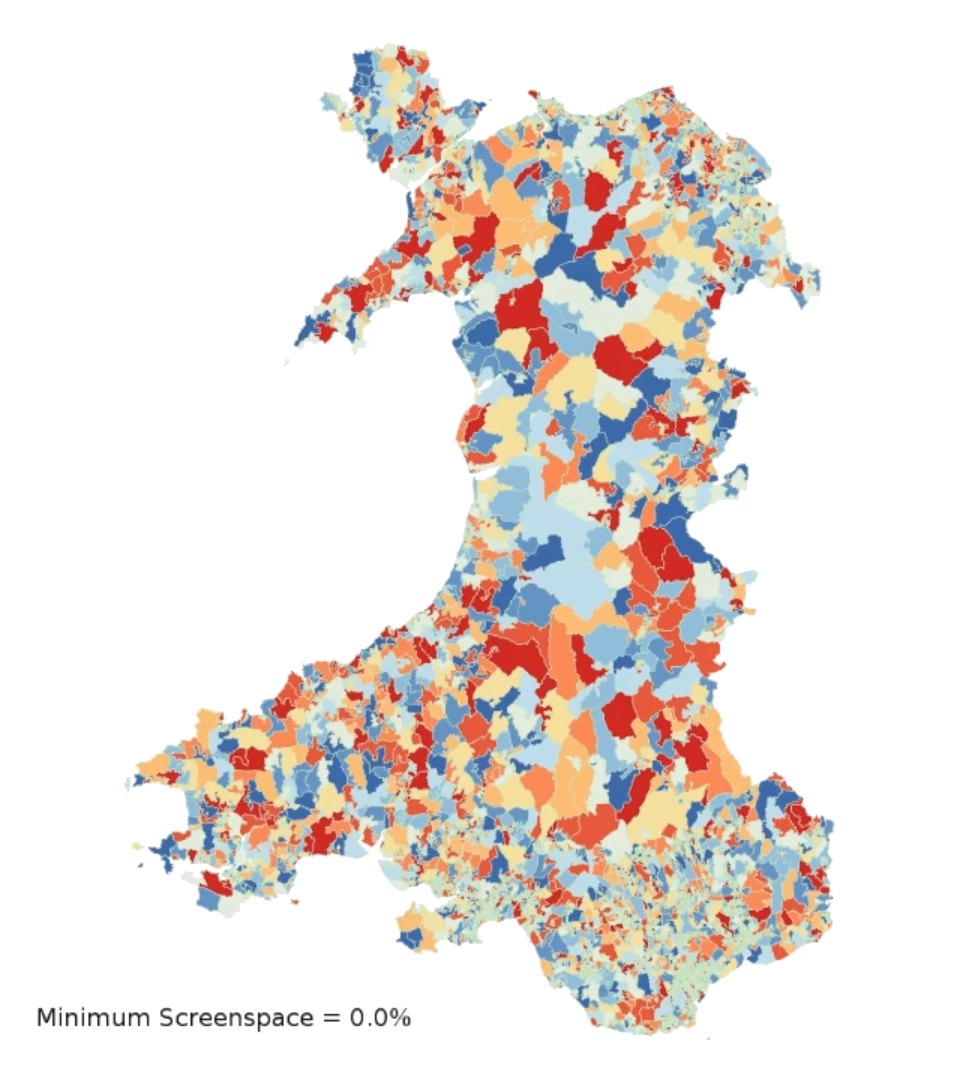
\includegraphics[width=0.5\textwidth]{images/ch3/compareA.png}}
\subfloat[]{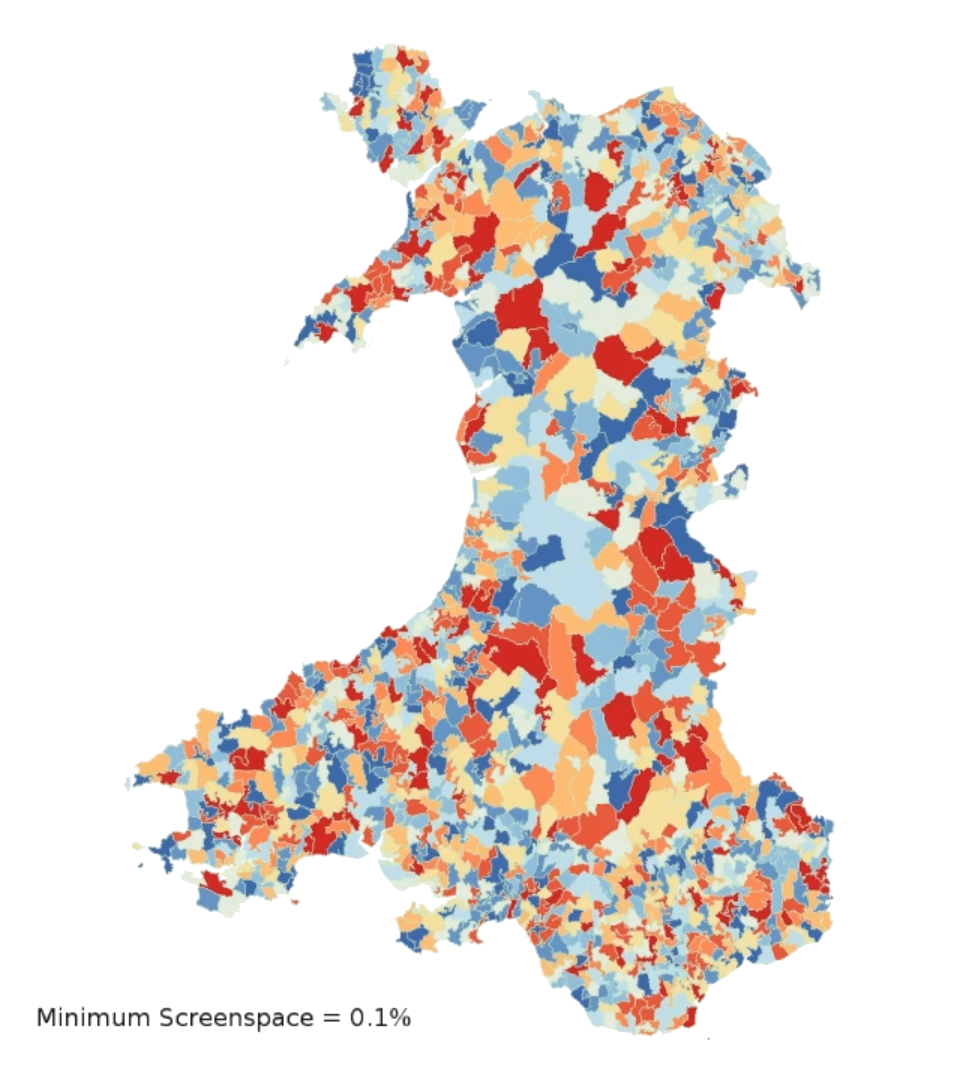
\includegraphics[width=0.5\textwidth]{images/ch3/compareB.png}}
\caption{A comparison of 2 different minimum screen spaces for the Lower Super Output Areas (LSOAs) of Wales. (a) depicts the original, un-editied map. (b) depicts an enforced screenspace minimum of 0.1\%.} \label{fig:compareA}
\end{sidewaysfigure}

\begin{sidewaysfigure}[p]

\subfloat[]{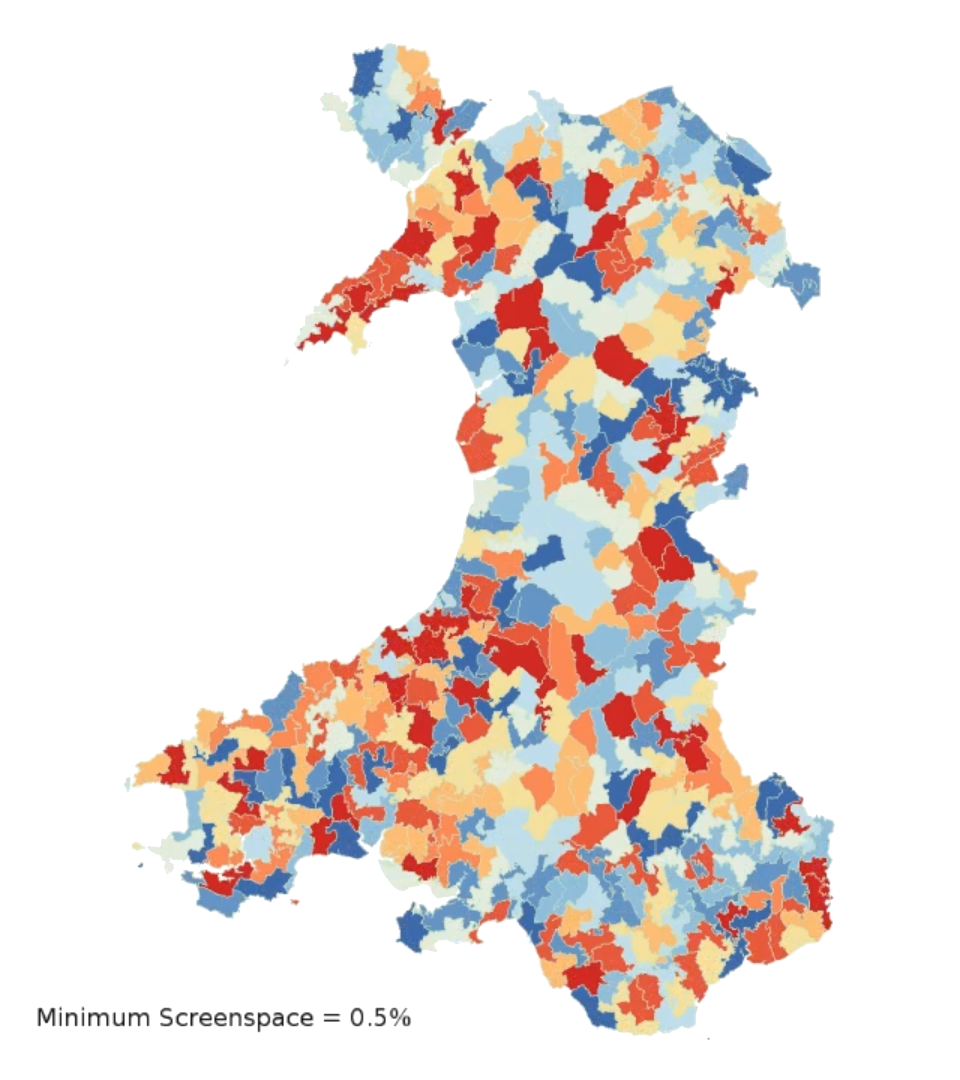
\includegraphics[width=0.5\textwidth]{images/ch3/compareC.png}}
\subfloat[]{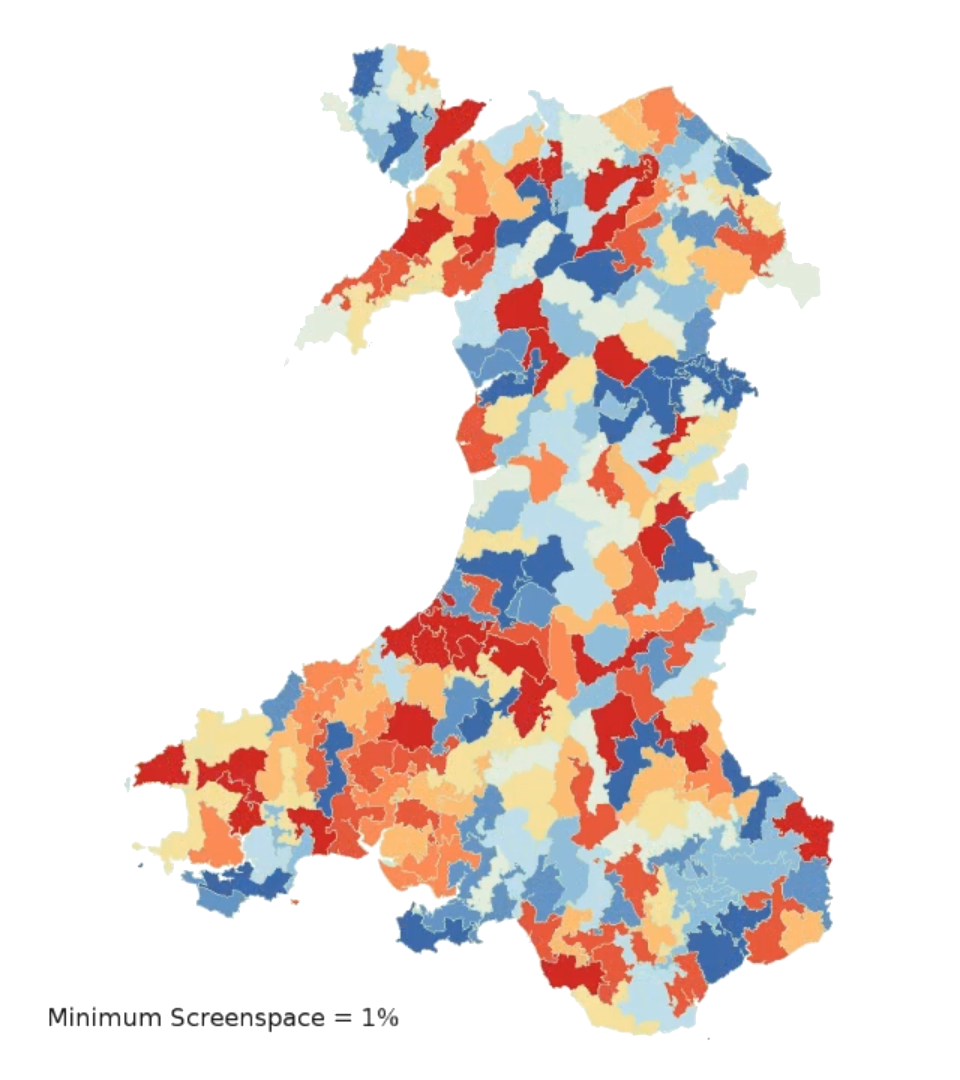
\includegraphics[width=0.5\textwidth]{images/ch3/compareD.png}}
\caption{A comparison of 2 more minimum screen spaces for the Lower Super Output Areas (LSOAs) of Wales (Refer to \ref{fig:compareA}). (a) presents an enforced minimum screenspace of 0.5\%. (b) presents an enforced screenspace .}
\end{sidewaysfigure}
